\RequirePackage{fix-cm}
%\documentclass{svjour3}                     % onecolumn (standard format)
%\documentclass[smallcondensed]{svjour3}     % onecolumn (ditto)
%\documentclass[smallextended]{svjour3}       % onecolumn (second format)
\documentclass[twocolumn]{svjour3}          % twocolumn

\smartqed  % flush right qed marks, e.g. at end of proof

\usepackage{amsmath}
\usepackage{amssymb}
\usepackage{xcolor}
\usepackage{algorithm}
\usepackage[noend]{algpseudocode}
\usepackage{graphicx}
\usepackage{csquotes}
\usepackage{listings}
\usepackage{hyperref}
\usepackage{array}

\journalname{Software and Systems Modeling}

% custom commands

\newcommand{\code}[1]{\small \texttt{#1}}

%\newcommand{\NOTE}[1]{\textcolor{red}{#1}}
\newcommand{\NOTE}[1]{}

\lstset{
	basicstyle=\scriptsize\ttfamily,
	keywordstyle=\color{violet}\bfseries,
	numbers=left,
	numberbychapter=false,
	xleftmargin=18pt
}


% Overleaf project: https://v2.overleaf.com/4826897137gcytcjpchpdv

\begin{document}

\title{Benchmarking Bidirectional Transformations: Applying the Benchmarx Framework to the Families-to-Persons Case\thanks{This paper is an extended version of \cite{Anjorin2017}.}}

\titlerunning{Benchmarking Bidirectional Transformations}  

\author{Anthony Anjorin \and Thomas Buchmann \and Zinovy Diskin \and Bernhard Westfechtel \and
	Romina Eramo \and Georg Hinkel \and Hsiang-Shang Ko \and Leila Samimi-Dehkordi \and Albert Z{\"u}ndorf
}

\institute{
	Anthony Anjorin \at
	Paderborn University, Germany\\
	\email{anthony.anjorin@upb.de}
	\and 
	Thomas Buchmann \at
	University of Bayreuth, Germany\\
	\email{thomas.buchmann@uni-bayreuth.de}
	\and
	Zinovy Diskin \at
	McMaster University, Hamilton, Ontario, Canada\\ 
	\email{diskinz@mcmaster.ca}
	\and
	Bernhard Westfechtel \at
	University of Bayreuth, Germany\\
	\email{bernhard.westfechtel@uni-bayreuth.de}
	\and 
	Romina Eramo \at
	University of L'Aquila, Italy\\
	\email{romina.eramo@univaq.it}
	\and
	Georg Hinkel \at
	FZI, Karlsruhe Institute of Technology, Germany\\
	\email{hinkel@fzi.de}
	\and 
	Hsiang-Shang Ko \at
	National Institute of Informatics, Tokyo, Japan\\
	\email{hsiang-shang@nii.ac.jp}
	\and
	Leila Samimi-Dehkordi \at
	University of Isfahan, Iran\\
	\email{samimi@eng.ui.ac.ir}
	\and
	Albert Z{\"u}ndorf \at
	University of Kassel, Germany\\
	\email{zuendorf@uni-kassel.de}	
}


\date{Received: date / Accepted: date}

\maketitle

\begin{abstract}
	\NOTE{\emph{Responsible: } Bernhard}
	
	Bidirectional transformations (bx) are relevant for a wide range of application domains. 
	While bx problems may be solved with unidirectional languages and tools, maintaining separate implementations of forward and backward synchronizers with mutually consistent behavior can be difficult, laborious, and error-prone. 
	To address the challenges involved in handling bx problems, dedicated languages and tools for bx have been developed. 
	Due to their heterogeneity, however, the numerous and diverse approaches to bx are difficult to compare, with the consequence that fundamental differences and similarities are not yet well understood. 
	This motivates the need for suitable benchmarks that facilitate the comparison of bx approaches.  
	
	This paper presents Benchmarx, a novel framework for evaluating bx tools that takes the heterogeneity of bx tools into account.
	The Benchmarx framework abstracts from technological spaces, specific tool architectures, and the internal data maintained by the tools.
	A benchmark for a specific bx problem is implemented by providing a suite of executable test cases. 
	By implementing a set of general interfaces, a solution to such a benchmark may then be developed using a specific bx tool and evaluated by executing the test suite. 
	
	To illustrate the use of the Benchmarx framework, we present a variety of solutions to the well-known Families-to-Persons benchmark, which involves synchronizing a database of families consisting of mother, father, daughters, and sons, with a database containing only unconnected male and female persons. 
	The solutions were selected to demonstrate how the Benchmarx framework supports the systematic comparison of considerably different approaches to solving bx problems, including procedural approaches using pairs of unidirectional transformations, approaches that suitably combine bidirectional primitives, and approaches that utilize a grammar-based or constraint-based consistency specification for consistency restoration.
	
	\keywords{Bidirectional Transformation \and Benchmark}
\end{abstract}


\NOTE{Notes that won't be part of the final text are in red.}
\NOTE{\emph{Estimated overall length:} 30--35 p. in two-column SoSyM format + references}

\clearpage

\section{Introduction}
\label{sec:Introduction}

\emph{Bidirectional transformations (bx)} are mechanisms for specifying and maintaining consistency between two or more artifacts.\footnote{In this paper we consider only the case of two artifacts.} 
Bx have been studied in many areas, including model-driven software development, graphical user interfaces, and transformations between heterogeneous data formats~\cite{ICMT2009-Czarnecki}.

While bx problems may be solved using unidirectional languages and tools, maintaining a separate implementation of different synchronizers with mutually consistent behavior can be difficult, laborious, and error-prone. 
In an attempt to better address bx-specific challenges, a variety of dedicated languages and tools for bx have been developed to assist software developers in solving bx problems more efficiently and reliably. 
Indeed, a wide spectrum of bx approaches has been reported in the literature, for example, by Hidaka et al.~\cite{SOSYM-Hidaka2016}, who provide a detailed, feature-based classification of numerous bx approaches and tools.

Due to their substantial heterogeneity, however, bx tools are difficult to compare with the consequence that fundamental differences and commonalities are still not well understood.
This situation hinders the development of better bx tools that combine the strengths and avoid the weaknesses of existing tools.
To promote the understanding of bx languages and tools, therefore, the need for bx \emph{benchmarks} was identified early~\cite{ICMT2009-Czarnecki}. 

As a first step towards this goal, a curated \emph{repository} of \emph{bx examples} was set up and is continuously being extended~\cite{Cheney2014}.
Subsequently, a proposal for additional requirements that a bx example must fulfill to become a bx benchmark was made~\cite{AnjorinCG0RS14}. 
%
Contrary to expectations, however, these preparatory activities and proposal did not result in any actual bx benchmarks.
We claim this is due to additional and substantial \emph{practical} challenges involved in setting up a bx benchmark that can be implemented with and executed for diverse bx tools.

This paper presents \emph{Benchmarx}~\cite{Anjorin2017}, a framework for bx benchmarks developed based on the conceptual work of Anjorin et al.~\cite{AnjorinCG0RS14}.
Benchmarx provides an infrastructure on top of which bx benchmarks can be implemented. 
In particular, the framework takes the heterogeneity of bx tools into account by abstracting from technological spaces, specific tool architectures, and the internal data maintained by the tools. 
A benchmark for a specific bx problem is implemented by providing a suite of test cases. 
Via a set of general interfaces, a solution to the bx problem developed using a specific bx tool can then be executed and evaluated using the provided test suite.  
Furthermore, the interpretation of test results is supported by identifying a set of tool features required by bx tests, thus enabling a fine-grained classification into expected and unexpected passed and failed test cases.
This enables a fair evaluation of specialized bx tools that can never pass all tests.

To provide a simple, but nonetheless non-trivial initial example of how to apply the Benchmarx infrastructure, the well-known \emph{Families-to-Persons} case was implemented as a bx benchmark and applied to a variety of bx tools. 
The Families-to-Persons benchmark, originally proposed as part of the ATL~\cite{SCP-Jouault2008} transformation zoo,\footnote{\url{http://www.eclipse.org/atl/atlTransformations/\#Families2Persons}} involves synchronizing a database of families consisting of mother, father, daughters, and sons, with a database containing a set of unconnected male and female persons with birthdays that cannot be inferred from the families database. 

We selected the Families-to-Persons case for several reasons: It is small and can be implemented in bx tools with acceptable effort. Furthermore, the data structures are simple and permit solutions using bx tools that operate on trees rather than on graph-like structures. 
Finally, despite its simplicity, it still poses a number of relevant challenges including heterogeneous data, loss of information, the absence of keys or any other form of identifiers, non-determinism, renaming and moves,\footnote{The exact meaning of a \emph{move} is defined for each case.} order-dependent update behavior, and a set of application-specific requirements to test for configurability of the bx tool.

To solicit a wide range of solutions, we submitted the Families-to-Persons benchmark as a case description to the Transformation Tool Contest 2017 (TTC 2017)~\cite{Anjorin2017a}.
Based on a selection of the solutions from TTC 2017, therefore, this paper is able to not only present the Benchmarx framework in detail, but also to compare and evaluate seven solutions to the Families-to-Persons benchmark developed with tools that differ considerably: 
\emph{BiGUL}~\cite{PEPM2016-Ko}, 
\emph{BXtend}~\cite{MODELSWARD2018-Buchmann}, 
\emph{eMoflon}~\cite{Leblebici2014a}, 
\emph{EVL+STrace}~\cite{IST2018-Samimi}, 
\emph{JTL}~\cite{SLE2010-Cicchetti}, 
\emph{NMF}~\cite{SoSyM2017-Hinkel}, and 
\emph{SDMLib}.\footnote{\url{www.sdmlib.org}}

This paper builds on several predecessor publications: the initial description of the Benchmarx infrastructure~\cite{Anjorin2017}, the description of the Families-to-Persons case for TTC 2017~\cite{Anjorin2017a}, and the presentation of some of the solutions discussed in this paper, also published as part of the TTC 2017 proceedings~\cite{Hinkel2017,Samimi-Dehkordi2017,Zundorf2017}. 
%
The current paper intends to underpin the following claims:

\begin{enumerate}
	\item The Benchmarx infrastructure is designed for implementing benchmarks to be executed by heterogeneous bx tools, which differ with respect to technological spaces, tool architectures, bx paradigms, and bx languages.
	\item The Benchmarx framework provides a classification of test cases that enables a useful interpretation of results for bx tools with a wide range of capabilities.  
	\item Comparing different solutions to the same benchmark assists in understanding the fundamental differences between bx approaches.
\end{enumerate}

The primary novel contribution of this paper is \emph{comparing and evaluating solutions implemented in bx tools covering a wide spectrum of bx approaches}.
This constitutes a crucial added value of this paper as previous publications essentially presented the Benchmarx infrastructure and individual solutions in isolation, failing to achieve this goal. 
After all, the need for comparing and evaluating diverse bx tools has been the driving force behind the Benchmarx initiative.

With respect to comparison and evaluation, we follow a \emph{qualitative} rather than a \emph{quantitative approach}. 
While we do collect and discuss metrics such as lines of code indicating (arguably) conciseness, number of (un)expected failed and passed test cases (measuring correctness), and run time (measuring performance), our primary goal is \textbf{not} to identify the ``best'' bx tool with respect to these metrics. 
We have to recognize that bx tools vary considerably with respect to their functionality and tool architecture. 
It is, therefore, problematic to compare tools that have been built for different purposes. 
We strive instead to explore the relationships between features of bx tools and properties of solutions developed with these tools. 
%
To this end, this paper is written in a neutral style and, in contrast to the spirit of the Transformation Tool Contest series, is not meant to imply a ranking among the solutions. 

This paper also contributes a \emph{conceptual framework for bx} which significantly extends our prior work~\cite{Anjorin2017}. 
This framework focuses primarily on \emph{architectures} of \emph{bx tools}, defined by their input and output data, the basic operations from which bx are composed, as well as their composition into different processing chains.  

The rest of this paper is structured as follows: Section~\ref{sec:Terminology} defines the terminology used throughout this paper. Section~\ref{sec:FamiliesToPersons} introduces the Families-to-Persons case, used as running example in all subsequent sections. 
Section~\ref{sec:Foundations} provides the conceptual foundations for our work. 
Section~\ref{sec:Benchmarx} describes the design of the Benchmarx framework. 
The solutions to the Families-to-Persons benchmark are presented in section~\ref{sec:Solutions}, together with an introduction and classification of the bx tool used to implement each solution. 
A comparison and evaluation of these solutions follows in section~\ref{sec:Evaluation}. 
Section~\ref{sec:RelatedWork} discusses related work, and section~\ref{sec:Conclusion} concludes the paper.

\section{Preliminaries:  Basic Terminology}
\label{sec:Terminology}

This section provides brief definitions for basic notions to be used throughout this paper. 
Additional, more specific terms will be introduced in more detail in section~\ref{sec:Foundations}. 
All notions are collected together in a glossary (appendix~\ref{sec:Glossary}). 
For a more comprehensive terminology and taxonomy for the domain of bx, the reader is referred to, e.g., Hidaka et al.~\cite{SOSYM-Hidaka2016}.

\subsection{Artifacts}
\label{sec:Artifacts}

Bidirectional transformations have been studied in a wide range of application domains. 
The \emph{artifacts} manipulated by them include, e.g.,\ data stored in databases, program data, and models. Throughout this paper, we will adopt terminology from model-driven software engineering~\cite{RodriguesdaSilva2015139} and refer to all artifacts as models. 

A \emph{model} is an abstraction of a system under study, which is more suitable than the system itself for certain purposes. 
A \emph{metamodel} is a model that defines the structure of a set of models, i.e., a modeling language.

For metamodeling, we employ \emph{Ecore} --- an implementation of Essential MOF, a subset of MOF~\cite{MOF-2.5.1}, provided by the Eclipse Modeling Framework (EMF)~\cite{steinberg09}. 
Although we present the Families-to-Persons benchmark using Ecore (section~\ref{sec:FamiliesToPersons}), bx tools do not have to be EMF-based to be able to implement the benchmark.

\subsection{Transformations} 
\label{sec:Transformations}

A \emph{transformation} reads, creates, or changes a set of $n \geq 1$ models.
A \emph{transformation definition} is a program that controls the execution of a transformation.

A \emph{bidirectional transformation (bx)} is a transformation that maintains consistency between a source model and a target model. 
The terms \emph{source model} and \emph{target model} are used to distinguish between the models involved in a bidirectional transformation; they do not imply a specific transformation direction.

\subsection{Synchronization}
\label{sec:Synchronization}

The act of executing a bidirectional transformation with the intent of establishing or maintaining consistency is denoted as \emph{synchronization}. 
Synchronizations may be classified along different dimensions.

A \emph{directed synchronization} operates on a \emph{master model} and a \emph{dependent model}, and is said to maintain consistency \emph{in the direction} of the dependent model. 
The master model is read, and the dependent model is created or changed to make it consistent with the master model. 
Required input for the synchronization can include the old master model, the exact changes applied to the master model, as well as preferences for making decisions during the synchronization process.  
A \emph{forward synchronization} is a directed synchronization in the direction of the target model; a \emph{backward synchronization} is performed in the opposite direction.

In contrast to a directed synchronization, both participating models have equal rights in a \emph{concurrent synchronization}. Thus, both source and target models may be changed to establish or maintain consistency.

A \emph{batch synchronization} is a directed synchronization that creates the dependent model from scratch. In contrast, an \emph{incremental synchronization} --- which may be directed or concurrent --- modifies an existing model.

A \emph{view-based synchronization} is performed between a model and a \emph{view} (an abstraction of the model that may be fully computed from the model). If neither model is a view of the other, the synchronization is \emph{symmetric}. 

An \emph{interactive synchronization} is partially controlled by user interactions performed during the synchronization. An \emph{automatic synchronization} can be run without any user interaction.

Finally, synchronization may be performed only \emph{on demand}, i.e., on explicit user request (e.g., via a dedicated synchronization command) or implicit user request (e.g., by saving a model to trigger synchronization implicitly).
In contrast, \emph{live synchronization} is performed immediately after each elementary change.  

\subsection{Consistency and bx laws}
\label{sec:Consistency}

A pair of source and target models is \emph{consistent} if both models agree on shared information. 
Consistency may be defined formally by a \emph{consistency relation} --- a relation that includes all pairs of related source and target models that satisfy some consistency condition. 
A consistency relation is \emph{deterministic} in the \emph{forward direction} if there is at most one consistent target model for a given source model; likewise for the \emph{backward direction}. 

A \emph{bx law} is a condition on the behavior of bidirectional transformations. 
The notion of a bx law is very strong: A bx language/tool satisfies a bx law only if the law is guaranteed to hold for every bidirectional transformation written in the respective language and executed in the respective tool. 
A number of bx laws have been proposed in the literature. 
In the following, we mention a few that are particularly relevant in the context of this paper. 
The reader should note that bx laws may be specific to certain classes of bx approaches and cannot be sensibly applied to all other approaches.

A bidirectional transformation is \emph{correct} if it produces consistent pairs of related models, and \emph{hippocratic} if it does not change models which are already mutually consistent \cite{SOSYM-Stevens2010}. Furthermore, a bidirectional transformation is \emph{stable} \cite{DBLP:journals/corr/PachecoMCV13}, if idle updates (no changes) to the master model always result in idle updates to the dependent model.
 
If the consistency relation is \emph{non-deter\-min\-is\-tic}, the correctness property does not determine the result of a bidirectional transformation in a unique way. 
In such cases, the principles of least change and least surprise aim at further determining desirable synchronization behaviour. 
A \emph{least change} transformation \cite{SOSYM-Macedo2016} restores consistency such that the changed model has a minimal distance to the original model (with respect to a suitably defined metric). 
A \emph{least surprise} transformation \cite{Cheney2015} behaves as closely as possible to users' expectations.

A \emph{round-trip law} states a property that refers to a round trip of directed synchronizations performed in sequence. 
For view-based synchronization, for example, an immediate recreation of the view must have no effect after a view update has been propagated to the model, and writing back an unmodified view must not change the model~\cite{TOPLAS2007-Foster}.

There are two more properties which are relevant for this paper: A bidirectional transformation \emph{terminates} if its execution halts after a finite number of steps. 
Finally, a bidirectional transformation is \emph{complete} if it has a well-defined domain on which it may be successfully executed.
Completeness is of practical relevance as some bx tools apply search-based heuristics that might not guarantee successful execution on all possible inputs.

\subsection{Bx tools}
\label{sec:BxTools}

A \emph{bx tool} is a tool for managing bidirectional transformations. It may be based on a \emph{bx language}, a domain-specific language for defining (programming) bidirectional transformations. 

The \emph{consistency relation} which a bx tool is supposed to maintain may be defined either explicitly or implicitly. An \emph{explicit} definition may be given, e.g., by a set of \emph{constraints} on pairs of related models \cite{QVT-1.3}, or by a \emph{grammar} \cite{Schurr1994} generating all consistent pairs of related models. 
In contrast, an underlying consistency relation may be implied only \emph{implicitly} by the steps required to establish or maintain consistency.

A bx tool may support different kinds of synchronization, according to the taxonomy introduced in section~\ref{sec:Synchronization}. 
Synchronization may be \emph{controlled} either \emph{explicitly}, by programming the steps to be executed for restoring consistency, or \emph{implicitly}, by deriving the steps automatically from other artifacts; forward (backward) synchronization may be derived from backward (forward) synchronization, or both directions may be derived from an explicit  consistency relation.

For model synchronization, a bx tool must in some way process changes between (old and new) model versions. Here, the term \emph{version} denotes a state of an evolving model at a specific point in time, defined by the model's contents. 
The general term \emph{change} subsumes any modification of the state of a model. 
A change may be represented by a \emph{delta}, i.e., a difference between two versions of the same model. 
Deltas may be classified further into \emph{structural deltas}, which are defined in terms of structural elements contained in both or only one of two model versions, and \emph{operational deltas}, which are composed of sequences of change operations applied to transition from an old to a new version of some model.

A bx tool may provide \emph{well-behavedness guarantees}, i.e., it may guarantee bx laws; see section~\ref{sec:Consistency}. 
Here, the term ``guarantee'' must be used with caution: The respective bx law must hold for each execution of each transformation definition. 
For example, a tool supporting view-based synchronization may guarantee round-trip laws, either by composing the transformation from well-behaved bidirectional primitives \cite{TOPLAS2007-Foster}, or by deriving one directed synchronization from its opposite \cite{PEPM2016-Ko}.

Finally, bx tools may be classified according to their underlying architecture. 
The \emph{architecture} of a \emph{bx tool} is composed of (i) its external interface, defined by required inputs and provided outputs, and (ii) its internal processing, defined by processing steps and their organization; this is handled in detail in section~\ref{sec:Foundations}.  

\subsection{Benchmarks}
\label{sec:Benchmarks}

Generally speaking, a \emph{benchmark} is a standardized test that serves as a basis for comparison or evaluation.\footnote{Merriam-Webster 2013} 
More specifically, a \emph{bx benchmark} is a benchmark tailored to the domain of bidirectional transformations. As mentioned already in the introduction (section~\ref{sec:Introduction}), our work targets comparison rather than evaluation, i.e., we are more interested in comparing bx tools and solutions implemented in these tools, rather than in an evaluation with the goal of identifying the ``best'' tool or solution. 
We use three criteria for comparison: \emph{functionality} (measured in terms of failed and passed test cases), \emph{conciseness} (measured in terms of the size of a solution), and \emph{performance}, measured in the run time required for executing test cases.



\section{The Families-to-Persons benchmark}
\label{sec:FamiliesToPersons}

\NOTE{\emph{Length:} 2 p., \emph{Responsible:} Bernhard}

%\NOTE{Based on TTC 2017, Section~2, or ENASE 2018, Section~3. Metamodels, functionality of batch and incremental transformations, challenges. Presentation of test cases, classified according to the developed taxonomy.}

In the Families-to-Persons benchmark, two related, but differently structured models have to be kept consistent: A \emph{families model} with parents and children, and a \emph{persons model} containing a flat set of males and females. 
Using the terminology introduced in the previous section, we present in this section the TTC 2017 variant of the Families-to-Persons case~\cite{Anjorin2017a,ENASE2018-Westfechtel}, which forms the basis of the benchmark reported in this paper. 

\subsection{Metamodels and consistency}
\label{sec:MetamodelsAndConsistency}

Figure~\ref{fig:metamodels} displays Ecore-based \emph{metamodels} for families and persons models, respectively.
Ecore-based bx tools implementing the benchmark may use these metamodels directly.
As the Benchmarx framework hides models behind data abstraction interfaces, any equivalent definition which is suitable for an implementing tool may be used instead (e.g., type definitions in a functional programming language (Haskell) for BiGUL).

\begin{figure}[tb!]
	\centering
	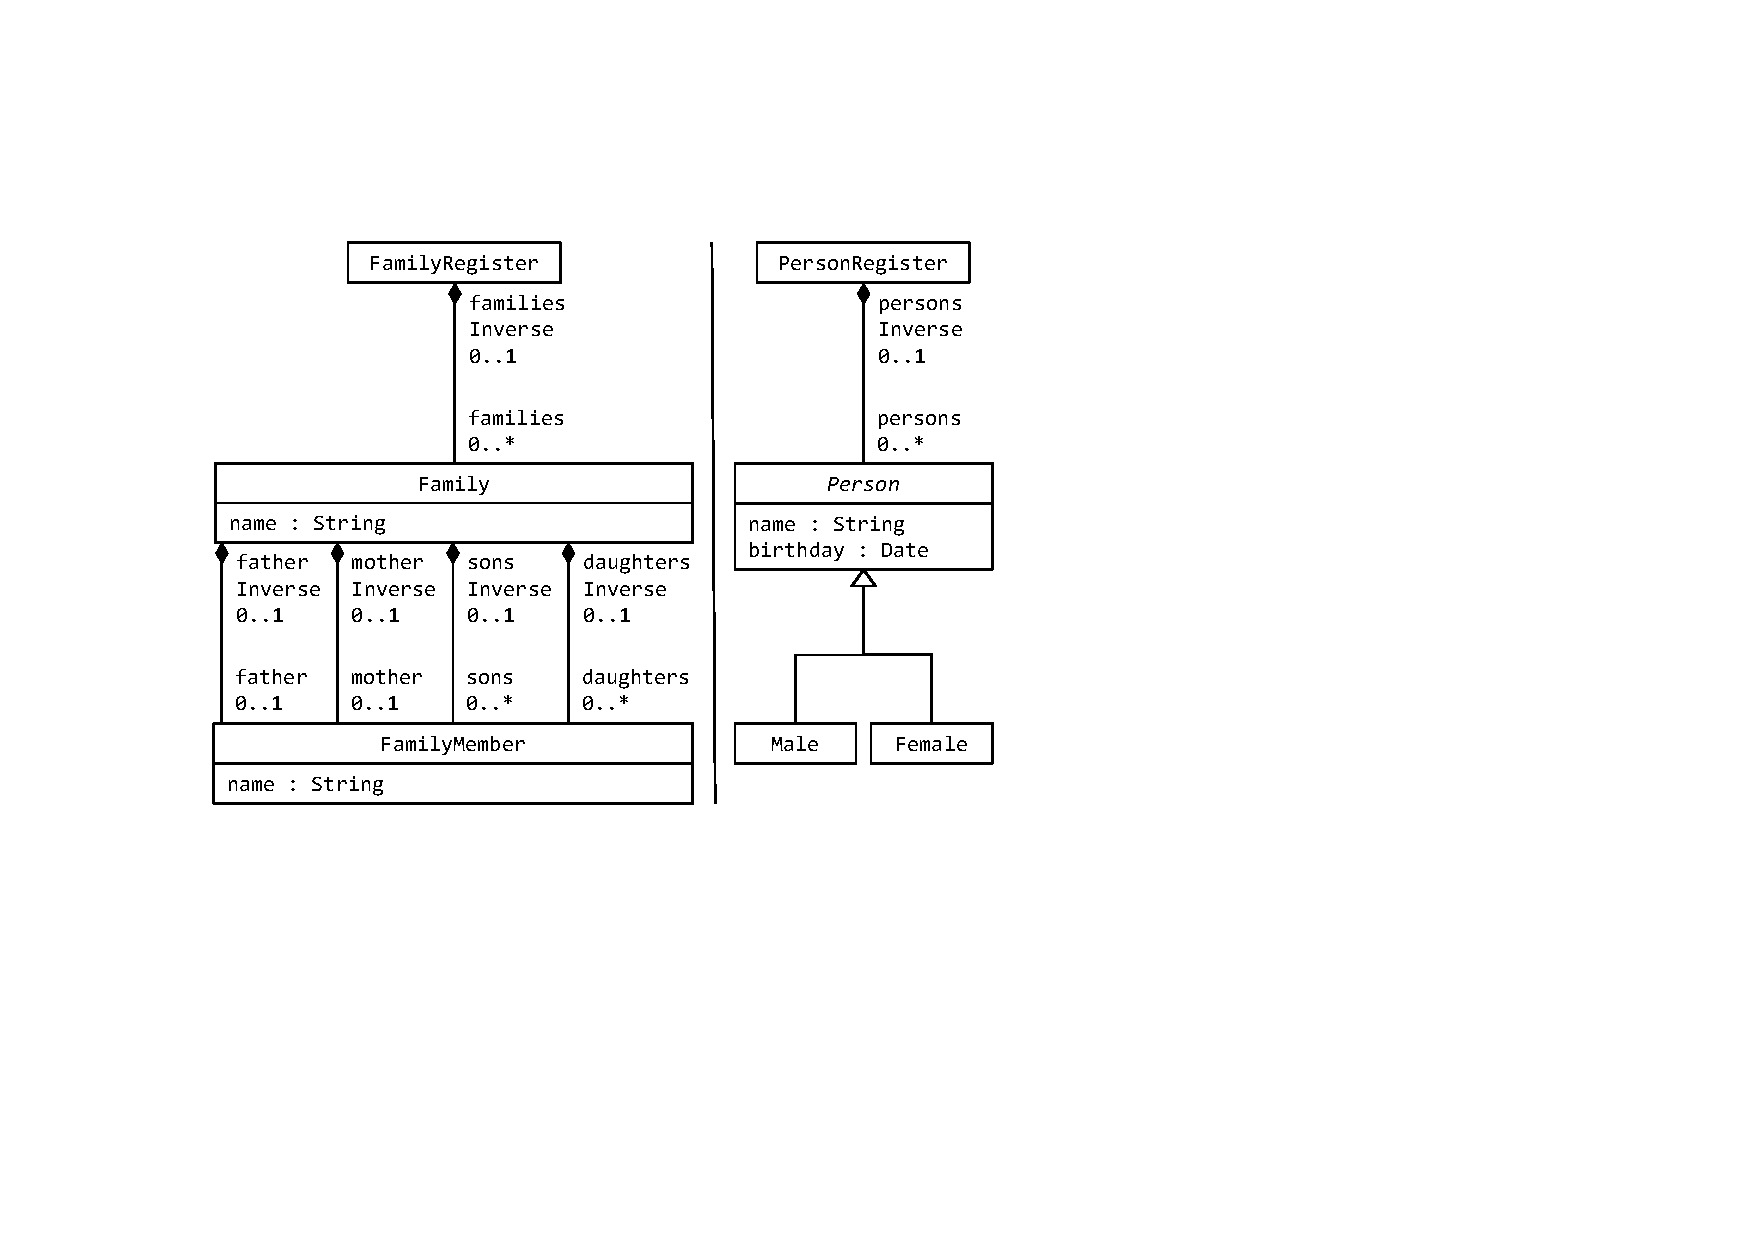
\includegraphics[width=\columnwidth]{diagrams/Metamodels}
	\caption{Metamodels}
	\label{fig:metamodels}
\end{figure}

\begin{figure*}[tb!]
	\centering
	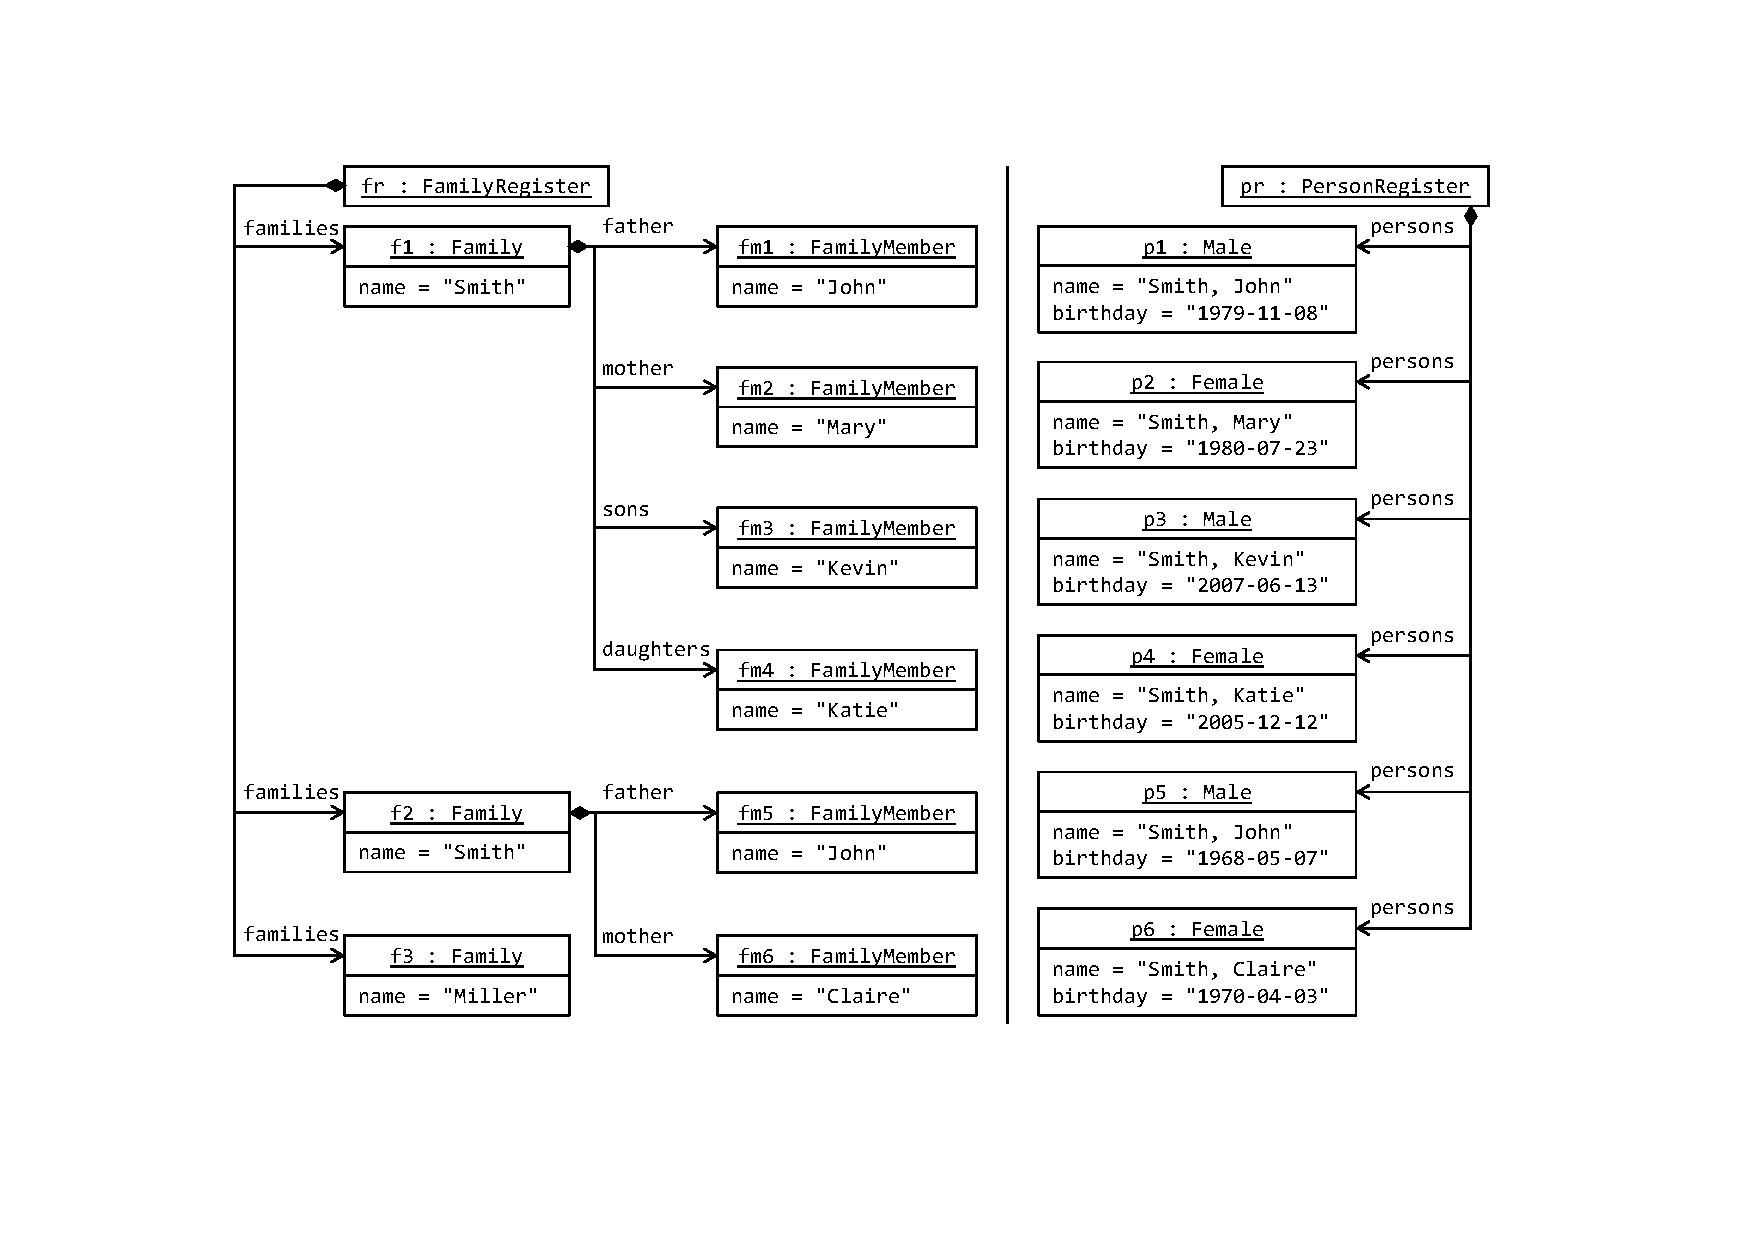
\includegraphics[width=0.75\textwidth]{diagrams/Models}
	\caption{Example of mutually consistent models}
	\label{fig:models}
\end{figure*}

We assume a unique root in each model (a family and a person register, respectively). 
A family register stores an unordered collection of families. 
Each family has members who are distinguished by their roles. 
The metamodel permits at most one mother and at most one father as well as an arbitrary number of daughters and sons. 
A person register maintains a flat unordered collection of persons who have a birthday and are either male or female. 
Note that key (combinations of) properties cannot be assumed in either model: There may be multiple families with the same name, family members with the same name even within a single family, and multiple persons with the same name and even the same birthday. 

A families model is \emph{consistent} with a persons model if a bijective mapping between family members and persons can be established such that:

\begin{enumerate}
	\item  Mothers and daughters (fathers and sons) are paired with females (males).
	\item  The name of every person $p$ is ``$f.name$,~$m.name$'', where $m$ is the member (in family $f$) paired with $p$.
\end{enumerate}

An example of mutually consistent models, conforming to the metamodels in figure~\ref{fig:metamodels}, is depicted as an object diagram in figure~\ref{fig:models}. 
To simplify the diagram, all inverse links (e.g., \code{familiesInverse}) are omitted.

The \emph{consistency relation} between families models and persons models is \emph{non-deterministic} in both directions: For a given families model, there are multiple consistent persons models (the birthdays may be chosen arbitrarily). Conversely, a given persons model is consistent with multiple families models (due to different groupings into families and different roles, e.g., mother or daughter).

%\subsection{Consistency Restoration According to Bx Laws}
\subsection{Synchronization}
\label{sec:ConsistencyRestoration}

%The family-to-persons benchmark is currently restricted to forward and backward consistency restoration.
%A forward (backward) consistency restorer can only change the target (source) model to restore consistency and is not allowed to change the current source (target) model.
%The exact details of the possible range of further input and output artifacts is discussed later in Section~\ref{sec:Foundations}. 
%

\subsubsection{Properties of synchronization}

The Families-to-Persons case is \emph{symmetric}~\cite{Diskin2014}, i.e., neither model is a strict view of the other and information loss may occur in both transformation directions. We consider only \emph{directed synchronization}, assuming that changes have been applied to the master model, while the dependent model has not been changed at all or the changes do not affect the consistency relation (e.g., changes of birthdays in the persons model are allowed). We cover both \emph{batch synchronization}, where the dependent model is created from scratch, and \emph{incremental synchronization}, where the dependent model is changed to restore consistency with the master model. Synchronization is performed  \emph{on demand} and \emph{automatically}.
Finally, changes are provided to the tools indirectly via an ordered\footnote{The results of some test cases depend on the order of elementary change operations.} sequence of change operations referred to as \emph{edits}.
%
%In the following, we classify synchronization properties 
%
%In the Families-to-Persons benchmark, the approach to \emph{consistency restoration} is characterized by the following properties:
%
%\begin{description}
%	\item[\textbf{Unidirectional consistency restoration}] Starting\\ from a consistent pair of source and target models, the source model is modified, and updates are propagated to the target model. Consistency restoration does not modify the source model; rather it reestablishes consistency by updating the target model.
%	
%	\item[\textbf{Operation-based update propagation}] Bx tools are provided with operational deltas, i.e., sequences of changes operations, which they need to propagate from the source to the target model.
%	
%	\item[\textbf{Propagation on demand}] Updates need to be propagated on demand only; bx tools are not required to perform live propagation, i.e., immediate propagation of each elementary change.
%		
%	\item[\textbf{Alternating updates}] It is assumed that the target model has not been modified at all while updating the source model, or the changes do not affect the consistency relation (e.g., changes of birthdays in the persons model are allowed).
%	
%	\item[\textbf{Batch and incremental transformations}] Con\-sist-\\ency restoration operates incrementally as it modifies an existing target model. Batch transformations are treated as a special case: Empty source and target models are taken as starting point; then, updates constructing the source model are propagated to the target model.
%	
%	\item[\textbf{No user interactions}] Consistency restoration operates automatically and does not involve any decisions to be performed interactively at runtime.
%\end{description}
%
These properties describe how the benchmark is designed but do not, however, prescribe the architecture of a bx tool that can be used to implement the benchmark (see section~\ref{sec:Foundations}).
For example, it is possible to execute the benchmark with a tool supporting live synchronization. Furthermore, a bx tool can apply the provided edits and decide either to record operational deltas, structural deltas, or just to use the old and new versions of the model.

\subsubsection{Bx laws}
\label{sec:BxLaws}

From the bx  laws introduced in section~\ref{sec:Consistency}, the benchmark takes \emph{correctness} into account by the design of the test cases: All test cases check for consistency by requiring a dependent model which is consistent with the master model. Similarly, \emph{termination} and \emph{completeness} are considered implicitly since violation of these properties would result in failed test cases.

Several test cases address \emph{hippocraticness} explicitly. In the benchmark, we consider the following type of hippocraticness: Starting with a consistent pair of a master model and a dependent model which have been synchronized before, the dependent model must not be changed if the changes to the master model do not affect the consistency relation. 

Although \emph{round-trip laws} are not considered explicitly in the benchmark, some are implied: If forward and backward synchronizers are correct and hippocratic, the forward (backward) synchronizer produces a consistent pair of models.
Furthermore, if the opposite synchronizer is invoked immediately, it will have no effect, due to its hippocraticness.
Additional tests for other round-trip laws such as \emph{putput} (well-behaved composition of forward (backward) synchronization) can be added in the future.

As mentioned earlier, the consistency relation between families models and persons models is non-de\-ter\-min\-istic in both directions.
In addition to bx laws such as correctness and hippocraticness, further guidance is needed to confine the possible choices in restoring consistency.
\emph{Least change} and \emph{least surprise} are useful principles to determine how the dependent model should be changed in a synchronization.
While we did take these principles into account, we came to the conclusion that they are not sufficient to derive the synchronization behavior in a unique way. 

We therefore describe the synchronization behavior explicitly, taking correctness, hippocraticness, but also the principles of least change and/or least surprise (as informal guidelines) into account. Furthermore, we refrain from a formal specification and provide an informal --- yet (hopefully) precise --- description of the expected behavior.
All test cases conform to and assert this description.
Formalizing these requirements is a task which we intentionally leave to the developers who implement the benchmark in a specific bx tool. 



%A variety of \emph{bx laws} have been proposed in the literature; see e.g.\ \cite{Cheney2015,Stevens2008c}. The Families-to-Persons benchmark takes the following laws into account:
%
%\begin{description}
%	\item[\textbf{Correctness}] Consistency restoration actually has to  produce consistent pairs of models, according to the definition given in section~\ref{sec:MetamodelsAndConsistency}. All test cases check for consistency by requiring a target model which is consistent with the source model.
%	\item[\textbf{Hippocraticness}] Hippocraticness means that the target model is not updated if is already consistent with the source model. More precisely, we consider an operational variant of hippocraticness: Starting with a consistent pair of a source model and a target model, propagation of any delta being composed only of operations not affecting the target model leaves the target model unchanged. Several test cases are dedicated to check this property.
%\end{description}
%
%It should be noted that our definition of hippocraticness differs from the state-based definition introduced in \cite{SOSYM-Stevens2010}: It is not required that bx tools may deal with independently constructed models and then check for consistency before restoration. Rather, the concept of \emph{synchronization dialogue} to be introduced in section~\ref{sec:Benchmarx} ensures that all synchronizations begin with a defined start state (consisting of a families model with an empty family register and a persons model with an empty person register, respectively). Bx tools may initialize internal data structures (e.g., correspondences) before the dialogue proceeds by propagating changes in forward or backward direction.
%
%\emph{Round-trip laws} have not been considered explicitly because they are implied: If forward and backward consistency restorers are correct and hippocratic, the forward (backward) consistency restorer produces a consistent pair of models. Furthermore, if the opposite restorer is invoked immediately, it will not change the original source model any more, due to its hippocraticness. Therefore, test cases for round-trip laws would not provide additional insights.
%
%As mentioned earlier, the consistency relation between families models and persons models is non-de\-ter\-min\-istic in both directions. Correctness and hippocraticness are not sufficient to determine the behavior of consistency restoration uniquely. Intuitively, we assume that changes are propagated as precisely as possible from the source to the target model, with minimal impact on the target model. However, there is no formalization of this property which is accepted generally and may be applied in all circumstances. Some authors view consistency restoration as an optimization problem, frequently referred to as \emph{least change} \cite{SOSYM-Macedo2016}. Others prefer a more relaxed approach, denoted as principle of \emph{least surprise} \cite{Cheney2015}.
%
%Without delving deeply into this issue, we observe that neither of these principles is sufficient to derive the behavior of consistency restoration in a unique way. In some way, however, consistency restoration has to be defined as precisely as possible. Unresolved non-determinism would not only make implementation of test cases much more difficult, it would also result in unpredictable behavior, which, as we believe, would violate the principle of least surprise.
%
%Therefore, we decided to specify consistency restoration explicitly, taking correctness, hippocraticness, but also the principles of least change and/or least surprise (as informal guidelines) into account. Furthermore, we refrain from a formal specification and provide an informal --- yet (hopefully) precise --- description of the expected behavior. All test cases conform to this description. Formalizing these requirements is a task which we intentionally leave to the bx tool users who implement the benchmark.
%
%Altogether, the behavior of consistency restoration is fixed through a requirements specification, which is constrained, but not totally fixed by the bx laws mentioned above. Thus, in general bx tools have to provide for \emph{flexibility}: Users of bx tools must be able to realize \emph{application-specific requirements}.
%
%
%%We now provide an informal description of how consistency is to be restored in both these directions, starting with an overview of basic well-behavedness ``bx laws'' proposed by Cheney et al. and Stevens~\cite{Cheney2015,Stevens2008c}, which were used to guide the choice of the desired synchronization behavior manifested in the benchmark as a test suite.
%
%%We require forward (backward) consistency restoration to be \emph{correct}, i.e., that the resulting source and target models be consistent.
%%In addition, we require \emph{hippocraticness}, i.e., that forward consistency restoration only change the target model if this is indeed necessary (consistency has not already been established).
%%In some cases, we also have to invoke the principle of least surprise as discussed by Cheney et al.~\cite{Cheney2015}.
%%There currently exists no formal characterization of ``least surprise'' that is applicable to all scenarios, and the test cases that rely on least surprise were defined by collaborating with multiple case and solution authors until a consensus was achieved.

\subsubsection{Synchronization behavior}      

In the following, we discuss the expected synchronization behavior for a series of ``small'' changes grouped according to model element (family, family member, person, \ldots) and then according to a limited set of change types (create, delete, update, move).
This overview is sufficient to provide a high-level intuition for the benchmark.
The actual test cases of course combine different changes and are more involved. However, the behavior of composite changes is \emph{induced} by the behavior of elementary changes.

\paragraph{Forward synchronization:}

In the forward direction, the persons model must be manipulated to be consistent with the changed families model.
Defining the expected synchronization behavior is straightforward because the families model is determined uniquely, with the exception of birthday attributes.
To resolve non-determinism, we require that a default value be assigned as the birthday of a newly created person.
With this resolution, forward synchronization is determinist.

\noindent Changes to \emph{families} should be processed as follows:

\begin{description}
    \item[\textbf{Creation:}]
    New families can be created and must be inserted into the family register.
    This has no effect on the target model, which should not be changed.
    
    \item[\textbf{Deletion:}]
    A family can be deleted together with all its family members.
    All persons corresponding to the deleted family members should be deleted.
    
    \item[\textbf{Update:}]
    A family can be renamed.  All persons corresponding to the family members in the renamed family should be renamed accordingly.
    
    \item[\textbf{Move:}]
    Families cannot be moved as there is only a single family register and the collection of families is unordered.
\end{description}

\noindent Changes to \emph{family members} should be processed in the following manner: 

\begin{description}
    \item[\textbf{Creation:}]
    New family members can be created and must be immediately added to a family.
    A new person of the same gender as the family member should be created and added to the person register.
    The person's name should be appropriately composed from the family member's family name and surname.
    The birthday of the person should have a default value (arbitrarily fixed by the benchmark). 
    
    \item[\textbf{Deletion:}]
    A family member can be deleted.  The corresponding person in the person register should be deleted.
    
    \item[\textbf{Update:}]
    A family member can be renamed.  The corresponding person should be renamed accordingly.
    
    \item[\textbf{Move:}]
    If a member is moved, different cases have to be distinguished.
    If the gender is retained, the corresponding person object should be preserved; otherwise, the person should be deleted, and a new person with a different gender is created whose attributes are copied from the old person. 
    A move within a family does not affect the corresponding person's name; a move to another family results in a potential update of the person's name.
\end{description}


\paragraph{Backward synchronization:}

In the backward direction, a person may be mapped either to a parent or a child, and persons may be grouped into families in different ways. As argued earlier, non-determinism should be resolved as far as possible. This may be achieved in different ways. A \emph{default transformation} would fix specific mapping options (e.g., all persons may be mapped to children and grouped into the same family if their family names agree). 


%Without configuration, backward consistency would be \emph{non-deterministic}: For a given persons model, there are multiple families models that would all be in line with correctness, hippocraticness and even least surprise. 

To provide for more flexibility, we decided to require a \emph{configurable} backward synchronization, to be controlled by an \emph{update policy}\footnote{In practice this could either represent run time user interaction or compile time design preferences.} that must set two Boolean parameters:
(i) \code{prefer\-Parent\-To\-Child} controls whether a person is to be mapped to a parent or a child (if both options are possible), and (ii) \code{prefer\-Existing\-To\-New\-Family} determines whether a person is to be mapped to a family member added to an existing family, or added to a newly created family containing only this single family member (again if both options are possible). 
If both parameters are set to true, the second parameter should take precedence: If the only existing family with a matching family name has no unoccupied parent role, the member is inserted into the family as a child (thus respecting (ii) and ignoring (i)).

It should be noted that the update policy does not resolve non-determinism completely.
For example, let us assume that persons should be added to existing families as children.
If we insert another person with family name \code{Smith} into the persons model depicted in figure~\ref{fig:models}, a corresponding member may be inserted either into family \code{f1} or into \code{f2}.
Furthermore, the update behavior may depend on the \emph{order} of change operations. For example, if persons should be added to existing families as parents, and two male persons with family name \code{Miller} are added to the persons model, the first person will be added as a father and the second person as a son. 

%Note that the update policy reduces non-determinism without eliminating it completely. 
%If  both configuration parameters are set to true, the resulting families model depends on the order in which persons are processed. 
%For example, in Figure~\ref{fig:models}, there are three candidates for the father role in the Smith family (recall that the collection of persons is unordered). 

\noindent Let us now consider change operations on \emph{persons}:
%
\begin{description}
    \item[\textbf{Creation:}]
    New persons can be created and must be added to the person register.
    A new family member with correct gender and name should be created in a suitable family in the family register.
    The update policy is consulted if it is possible to add the new family member to an existing family, and if the family member can be added as a parent or a child.
    
    \item[\textbf{Deletion:}]
    Persons can be deleted.
    The corresponding family member should be deleted. 

    \item[\textbf{Update:}]
    Changes of birthdays do not affect the families model. 
%
    The first name of a person can be changed; 
    the name of the corresponding family member should be updated accordingly. 
%
    The family name of a person can be changed; 
    this change should not affect the current family and its members.
    The family preserves its name even if it does not contain any other members.
    The corresponding family member should instead be moved to another family, which may have to be created as required; the precise update behavior, if there are multiple possibilities, depends on the update policy.
    
    \item[\textbf{Move:}]
    Persons cannot be moved because the persons model consists of a single, flat, unordered collection. 
\end{description}

The update policy constitutes an example of \emph{ap\-pli\-ca\-tion-specific requirements}, as discussed at the end of section~\ref{sec:BxLaws}. The rules for handling changes to family names are application-specific, as well. They are based on the underlying assumption that the person intends to leave their family (e.g., because of marriage).
This kind of synchronization behavior may (arguably) be considered reasonable; we simply take it for granted, being required by an (imaginative) customer.
However, in certain circumstances it may (arguably) violate principles such as least change (e.g., if the person was the single member of a family); we use these principles only as general guidelines, not as strict laws. 


\subsection{Challenges}
\label{sec:Challenges}

The Families-to-Persons case includes a number of diverse \emph{challenges} summarized in the following:

\begin{description}
	\item[\textbf{Heterogeneous metamodels:}] 
	Solutions must establish a mapping between heterogeneous metamodels, where the same information is represented in different ways (concerning, e.g., names and genders).
	
	\item[\textbf{Loss of information:}] 
	The scenario is symmetric as the family structure is only present in the source, and birthdays are only present in the target.
	
	\item[\textbf{No keys:}] 
	There are no uniquely identifying (combinations of) properties for family members or persons, which makes synchronization difficult.
	
	\item[\textbf{Non-determinism:}] 
	The consistency relation is not de\-ter\-mi\-ni\-stic: For a given families model, there can be multiple correct persons models (birthdays may be arbitrarily selected). 
	Likewise, for a given persons model there can be multiple correct families models (due to different groupings into families and different roles in these families). Synchronization has to deal with this non-determinism (and resolve it as far as possible).
	
	\item[\textbf{Configurability:}] 
	The behavior of backward synchronization is controlled by an update policy determining roles of members and groupings of members into families. 
	The update policy may be changed at run time and should take effect only for future updates (no global reshuffling of the families model after the update policy has been changed).
	
	\item[\textbf{Renaming and movement:}] 
	Changes to be synchronized include not only creations and deletions, but also renamings and moves, which must not be reduced to deletions and creations so that changes can be synchronized in a minimally invasive way. 
	
	\item[\textbf{Order-dependent synchronization:}] 
	Backward synchronization depends on the order in which change operations on the persons model are processed. 
	For example, if two persons of the same gender are to be inserted into the same family as parents, only the first person can be inserted as a parent; the second person must be added as a child.
	
	\item[\textbf{Specific least surprise requirements:}]~
	The bench\-mark requires adherence to a case-specific definition of what ``least surprise'' is to mean.
	For example, if the family name of a person is changed, the corresponding family member should be moved to another family (rather than having the family name updated, with possible side effects on other members).
	This definition of which change is ``better'' or ``smaller'' than another is arguably arbitrary and must be treated as an additional requirement.
\end{description}

\section{Foundations}
\label{sec:Foundations}

\NOTE{\emph{Length:} 2 p., \emph{Resonsible:} Tony}

\NOTE{Based on BX 2017 paper, Section~3.1. Should include the taxonomy of Figure~3.}

\section{The Benchmarx Framework}
\label{sec:Benchmarx}

%\NOTE{\emph{Length:} 2 p., \emph{Responsible:} Thomas}
%
%\NOTE{Overview of the framework, provided components, approach to tool integration, synchronization dialogues, design and classification of test cases, execution of test cases.}
%\subsection{Overview}

\begin{figure}[tb!]
	\centering
	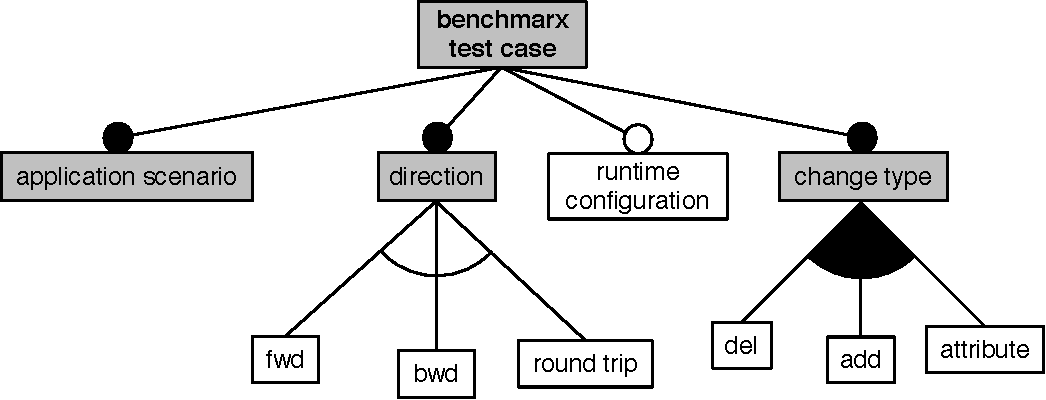
\includegraphics[width=\columnwidth]{diagrams/framework/feature-model-benchmarx-test-case}
	\caption{Variability of benchmarx test cases}
	\label{fig:featureModelBenchmarxTestCase}
\end{figure}

\begin{figure*}[tb!]
	\centering
	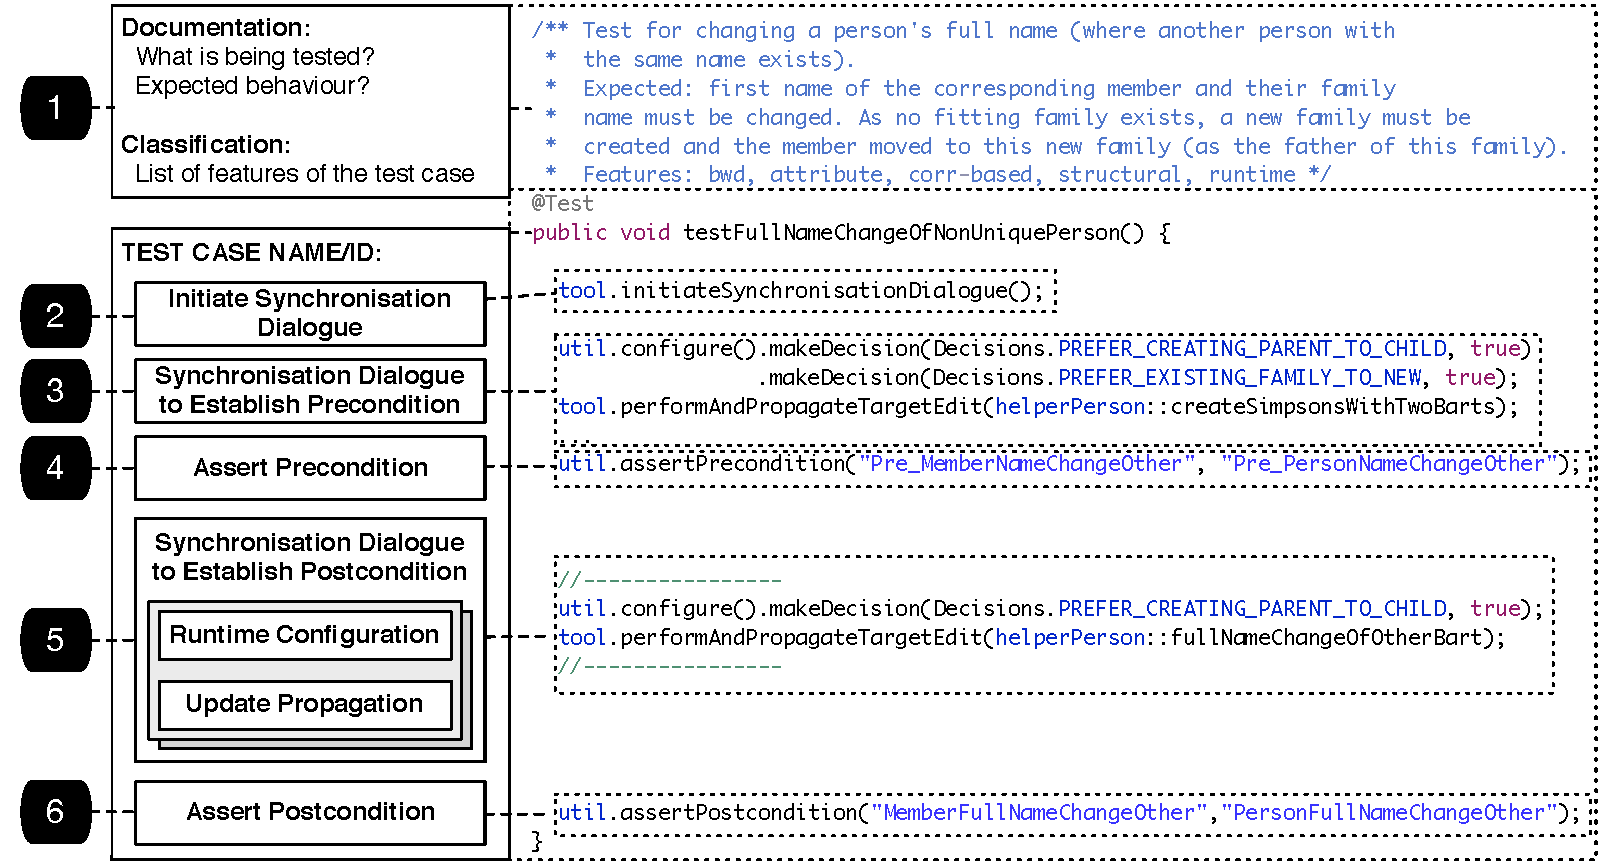
\includegraphics[width=0.75\textwidth]{diagrams/benchmarx/testCase}
	\caption{A benchmarx test case as a synchronization dialog}
	\label{fig:benchmarxTestCase}
\end{figure*}



The Benchmarx framework is a component-based framework allowing for a comparison of arbitrary bx tools. 
A major challenge that must be addressed by the framework is that different bx tools may require different input data. 
The Benchmarx framework must thus provide a unifying design space, in which different bx tool architectures can be placed, classified, and evaluated. 



While the general conceptual design of the Benchmarx framework can be transferred to any technological space, we provide a reference implementation based on Eclipse, the Eclipse Modeling Framework (EMF), JUnit as a unit testing framework, and Java.
To ensure that non-EMF and even non-JVM-based bx tools can be integrated with no restrictions on the input data of the tools, we use a string representation of produced and expected models established by convention for each benchmark example.
The current solutions to the Families-to-Persons case show that it is indeed possible to integrate diverse bx tools with reasonable effort.

\subsection{Design of a benchmarx test suite}
\label{sec:DesignOfABenchmarxTestSuite}

\begin{figure*}[tb!]
	\centering
	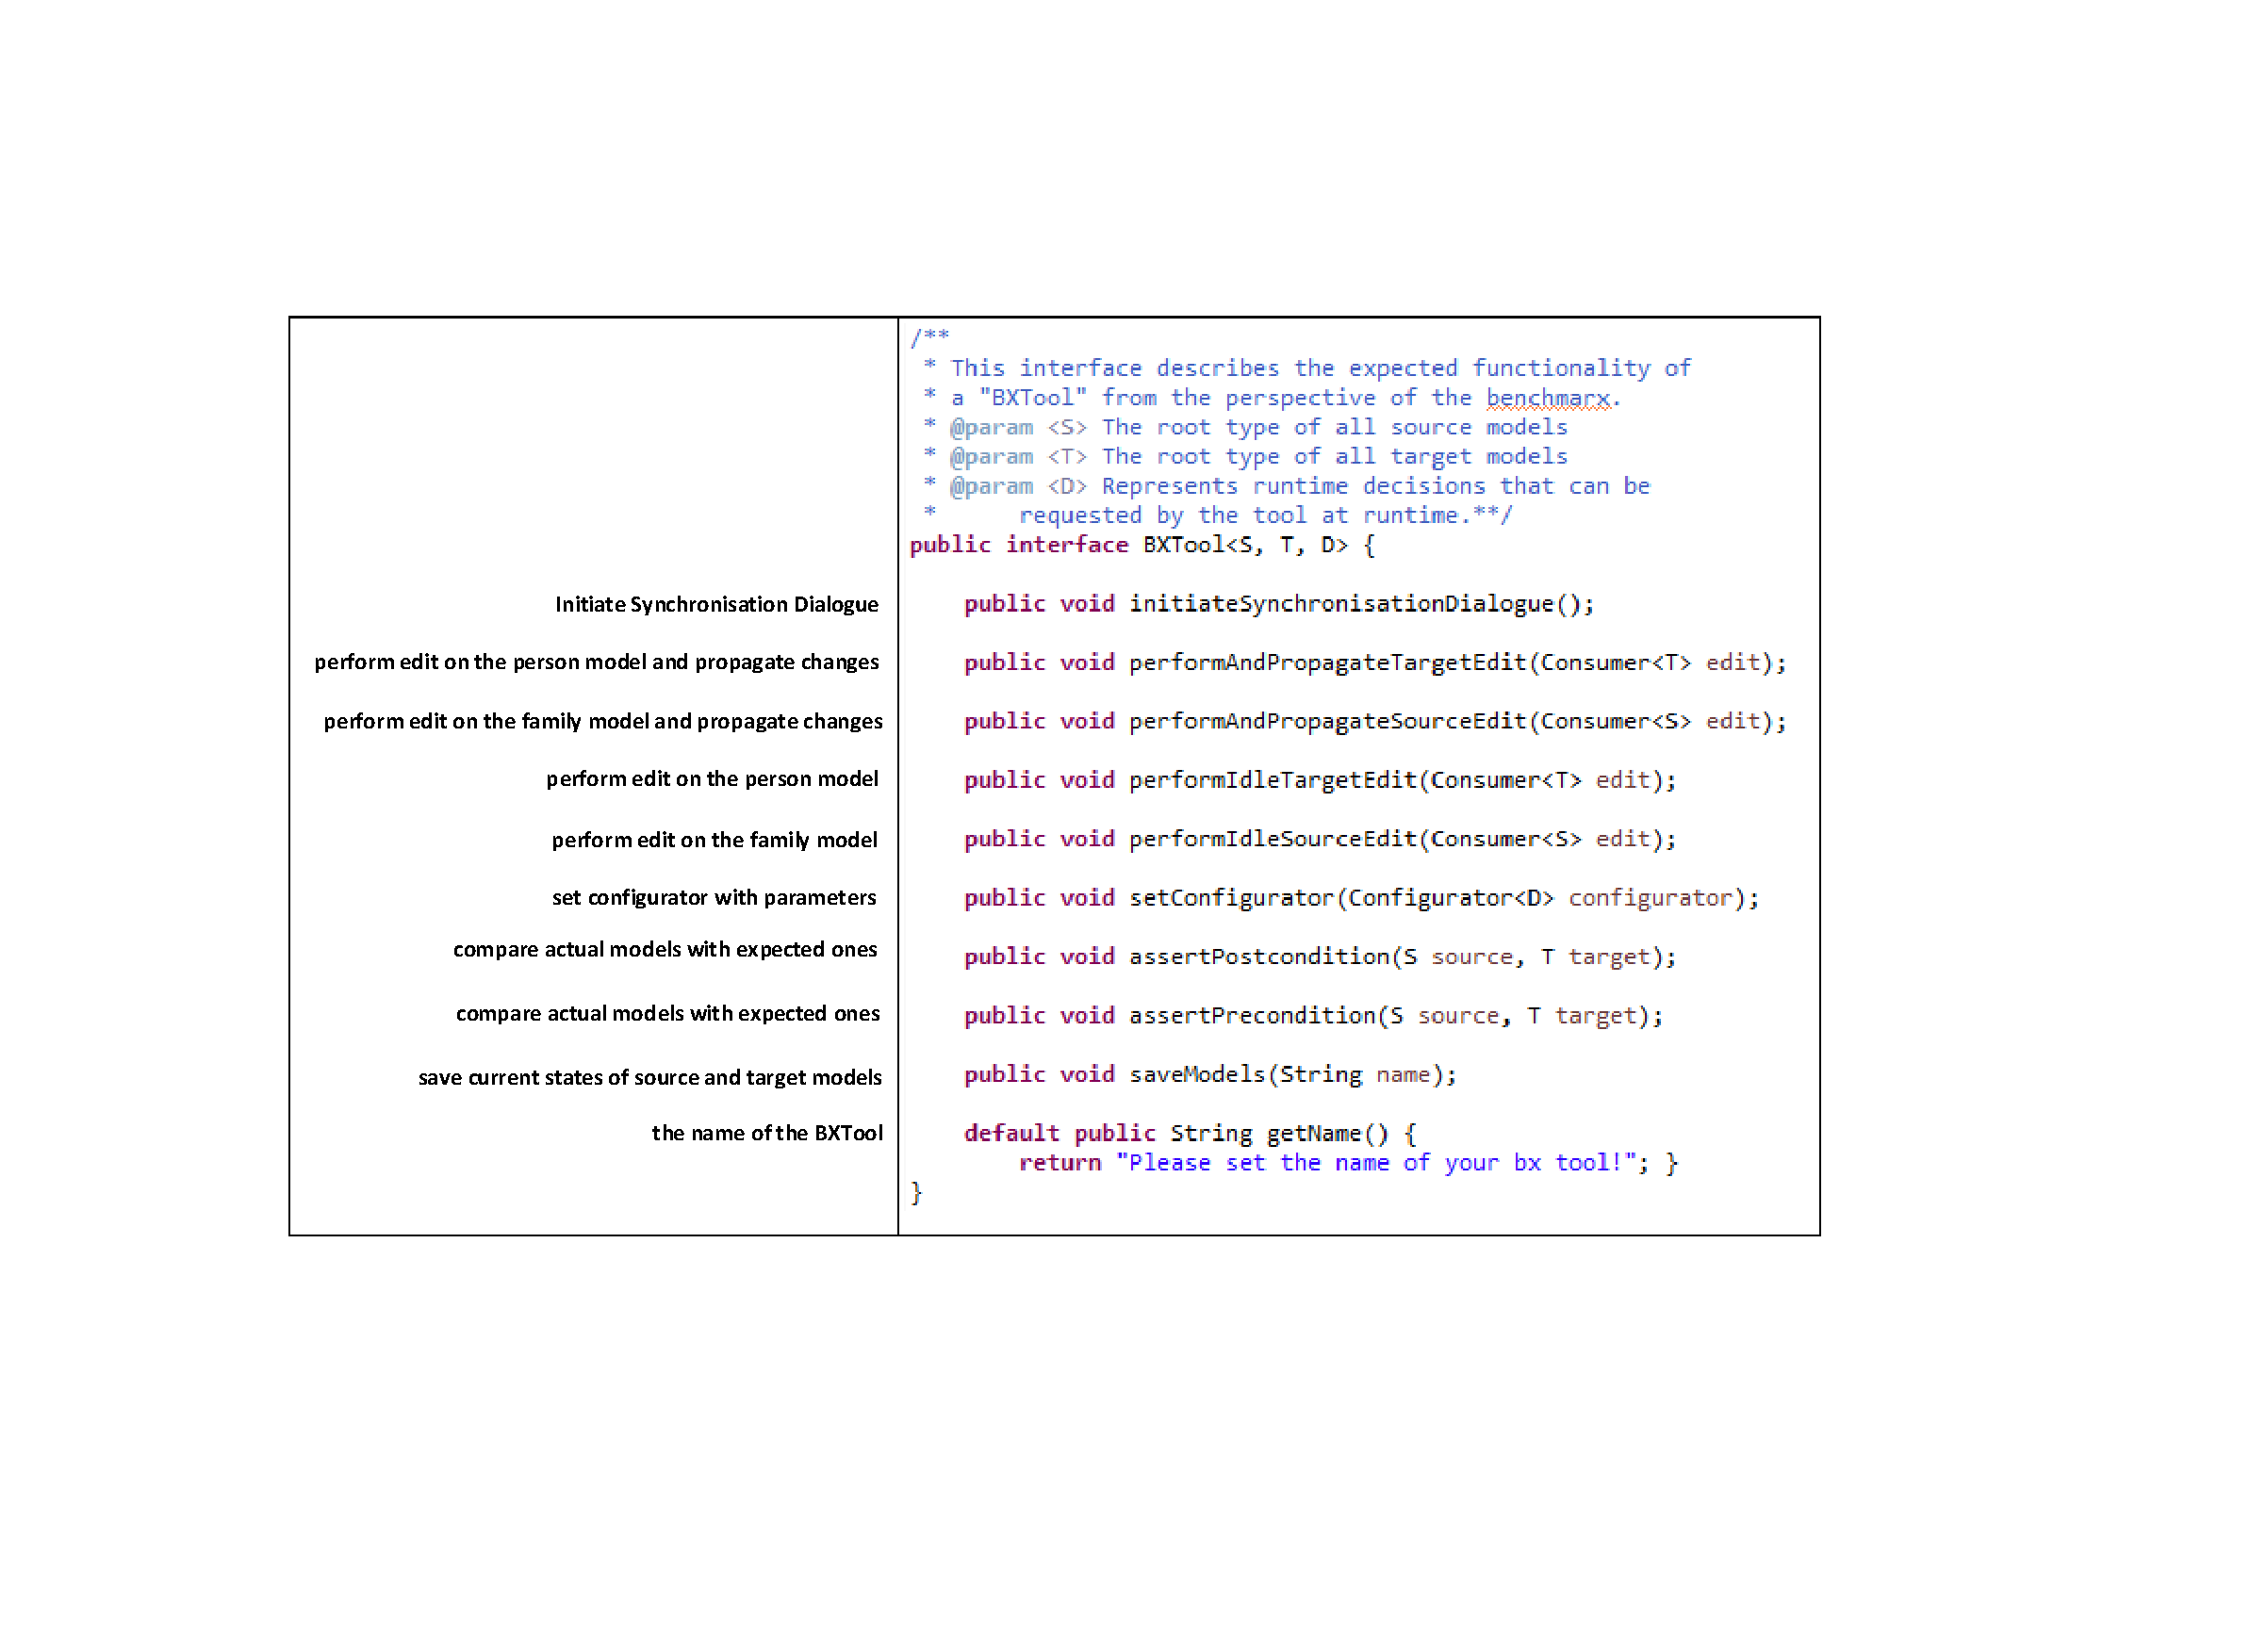
\includegraphics[width=0.75\textwidth]{diagrams/benchmarx/BXTool}
	\caption{The BXTool interface}
	\label{fig:refImplementation}
\end{figure*}

Figure \ref{fig:featureModelBenchmarxTestCase} depicts a feature model for benchmarx test cases. 
Every benchmarx test case must state the relevant application scenario (cf. Figure~\ref{fig:featureModelBxTools}), its direction to be (exclusively) \emph{fwd} (forward), \emph{bwd} (backward) or a mix of both, i.e., a \emph{round trip}, if the test case requires \emph{runtime configuration} or not, and the combination of different change types applied in the test. 
The set of possible change types can be extended in the future to accommodate more expressive frameworks. 

Benchmarx is designed as a generic framework for benchmarking bx tools; we thus strive to minimize requirements regarding the typically tool-specific representation of deltas and corrs. 
Instead of establishing some standard data structure for deltas and corrs, test cases are designed as \emph{synchronization dialogs}. 
A synchronization dialog always starts from the same agreed upon initial consistent state, and then applies a sequence of edits to the source and target models. 
Only the resulting models are directly asserted by comparing them with expected versions.
In this manner, each bx tool is free to maintain arbitrary internal state, e.g., recording deltas during edit application, or maintaining corrs in whatever format is required.

A benchmarx test case is depicted schematically to the left of Figure \ref{fig:benchmarxTestCase}, with a concrete test case for our example depicted to the right of Figure~\ref{fig:benchmarxTestCase}, following the proposed schema using JavaDoc, Java, and JUnit as implementation technologies.
Each test case contains a documentation (cf. label~1 in Figure~\ref{fig:benchmarxTestCase}) stating (i)~what is being tested, (ii)~the expected behaviour, and (iii)~a list of the concrete features of the test case taken from Figure~\ref{fig:featureModelBenchmarxTestCase} to clarify at a glance if a given bx tool can be expected to pass the test or not, i.e., if the relevant application scenario for the test case matches the addressed application scenario of the (implemented solution with the) bx tool. 

The test case itself starts by initializing the bx tool which is being tested (label~2); the agreed upon starting state is hereby established (e.g., for the Families-to-Persons benchmark this comprises a single empty family register and a corresponding single empty person register), and all necessary internal (auxiliary) tool-specific data structures can be created.

%%%%% TONY is here %%%%%>

The subsequent part of a test case (label~3) consists of a series of propagation steps, used to establish the precondition of the test. 
Although this creates a dependency on other tests (asserting exactly this precondition), it allows us to abstract from any tool-specific corr representation, as every bx tool can build up whatever internal state it requires along with the precondition. 
In this manner, the input corr is ``passed'' implicitly to the bx tool via a series of preparatory propagation steps.
Each propagation step is specified in the test case as a source or target edit (realized as a Java lambda expression), which is passed to the bx tool and is to be performed on the source or target model.
In this manner, the bx tool can record\footnote{EMF supports this via a notification framework.} whatever it wants when applying the edit to produce, e.g., a tool-specific representation of an o-delta or s-delta.

The precondition is finally asserted (label~4), representing a well-defined starting point for the test. 
If the test requires a runtime update policy (cf. section~\ref{sec:Introduction}), this is configured (label~5) just before propagating the relevant input edit.
A sequence of such (optional) configuration and edit propagation steps form the primary synchronization dialogue used to establish the postcondition (label~5).
The final part of a test case (label~6) is an assertion of the postcondition, checking if the final source and target models are as expected. 



In the concrete test case depicted to the right of Figure~\ref{fig:benchmarxTestCase}, a number of persons are created in the person register and then propagated backward to establish a consistent family register that is asserted as a precondition. 
As part of the actual test, a person named \texttt{Simpson, Bart} is now renamed in the person register; this change is propagated backward with a runtime update policy set to prefer creating parents (if possible) to creating children. 
Note that in this particular test, two persons with the name \emph{Bart Simpson} are created as part of the precondition (indicated by the target edit \texttt{createSimpsonsWithTwoBarts}). 
As a consequence, this test can only be reliably passed if corrs are exploited as explicit input (indicated by the feature \texttt{corr-based} in the classification of the test). 

The current test suite provided for the Families-to-Persons case consists of such test cases as in Figure~\ref{fig:benchmarxTestCase} separated into two broad categories: (1)~\emph{batch} test cases providing only the input model and no horizontal input (initial-batch-based), and (2)~\emph{alignment-based} test cases providing an input delta and input corr (delta-corr-based).
More tests covering the other bx application scenarios identified in Figure~\ref{fig:architectureLandscape} can be added in the future.
Each category comprises test cases for each transformation direction.\footnote{Recall from section~\ref{sec:Introduction} that the \emph{forward} direction is from the Families model to the Persons model, while \emph{backward} is from the Persons model to the Families model.}

While the batch test cases are basic tests used to check if a given source model is transformed into a new target model correctly, different input source deltas are handled by the alignment-based tests. 
In particular, renaming, deleting, and moving persons and family members are currently addressed in these test cases. 
To keep the number of test cases manageable, only the batch category contains separate test cases for each combination of configuration parameters.
In the alignment-based category, the parameters (preferences represented by the update policy) are changed dynamically during test case execution.



\subsection{Implementing a benchmark with a bx tool}



In order to use a specific bx tool with the benchmarx framework, a single interface \code{BXTool}, depicted and described in Figure~\ref{fig:refImplementation}, needs to be implemented.
For EMF-based tools, we provide an abstract class \code{BX\-Tool\-For\-EMF} that contains implementations for both \code{assert} methods and can be subclassed to simplify the integration in the benchmark.

The method \code{initiate\-Synchronisation\-Dialogue} is invoked before each test case run and is used to establish the agreed upon common starting state for a given benchmark.
For the Families-to-Persons case, this consists of a single empty family register and its corresponding single and empty persons register, plus all internal, tool-specific internal data structures. 

The methods \code{perform\-And\-Propagate\-Source\-Edit} and \code{perform\-And-Propagate\-Target\-Edit} are called from the test cases when corresponding edits should be performed and propagated on the corresponding models. 
In contrast, the methods \code{per\-form\-Idle\-Source\-Edit} and \code{per\-form\-Idle\-Target\-Edit} are used to modify source and target models, respectively, without propagating the change.
These methods should be used whenever a change in the respective models does not affect the opposite model, e.g., when the birthday date of a person is changed, or the role of a family member within its containing family.

Multiple benchmarks including Families-to-Persons, together with solutions using numerous bx tools are maintained in the benchmarx GitHub respository\footnote{\url{https://github.com/eMoflon/benchmarx}} together with documentation on how to add solutions to existing benchmarks as well as add entirely new benchmarks to the collection.

\section{Solutions}
\label{sec:Solutions}

\NOTE{\emph{Length:} 15 p., \emph{Responsible:} Bernhard for introductory paragraph, solution experts for the subsections}

\NOTE{One subsection (2 p.) for each tool. Presentation of (fragments of) the solution. Underyling concepts and paradigms are more important than technical details of the solutions. Code fragments serve as illustration and must be explained thoroughly.}

This section presents seven diverse bx tools all used to implement the Families-to-Persons benchmark.
A summary of a classification of these seven tools based on our feature model for bx tools is provided in table~\ref{tab:features-all-tools}.
In the following subsections, one for each tool/solution in alphabetical order, we shall refer to this table and explain each tool's classification in detail.

\newcolumntype{P}[1]{>{\centering\arraybackslash}p{#1}}
\newcolumntype{M}[1]{>{\centering\arraybackslash}m{#1}}
\begin{table*}[!tbp]
\begin{tabular}{M{1.7cm}|M{1.7cm}|M{1.7cm}|M{1.7cm}|M{1.7cm}|M{1.7cm}|M{1.7cm}|M{1.7cm}}
\textit{} & \textbf{BiGUL} & \textbf{BXtend} & \textbf{eMoflon} & \textbf{EVL + STrace} & \textbf{JTL} & \textbf{NMF Sync.} & \textbf{SDMLib} \\ \hline
\textit{Style} & CR (hAln) & CR &  &  &  &  &  \\ \hline
\textit{Scenario} & initial-state-based & initial-diag-based &  &  &  &  &  \\ \hline
\textit{Guarantees} & round-trip laws & none &  &  &  &  &  \\ \hline
\textit{Consistency} & implicit & implicit &  &  &  &  &  \\ \hline
\textit{Sync.} & on-demand, explicit and implicit & on-demand, explicit &  &  &  &  &  \\ 
\end{tabular}
\caption{Summary of classification of all tools and solutions}
\label{tab:features-all-tools}
\end{table*}

\subsection{BiGUL}
\label{sec:BiGUL}

\NOTE{\emph{Solution expert:} Josh, \emph{Interviewer:} Tony}

% History, website, tutorial, community
BiGUL~\cite{PEPM2016-Ko}, short for \emph{the Bidirectional Generic Update Language}, is the current result of a long line of research on \emph{bidirectional programming}~\cite{Foster2012} predominantly performed by the programming language community.
Bidirectional programming languages typically share two main ideas in common:  (i)~the task of programming a bx can be reduced by automatically deriving one direction of synchronization from the other direction that is explicitly programmed, and (ii)~well-behavedness properties are guaranteed by providing a small set of well-behaved primitive functions, and combinators to allow bx programmers to compose complex, well-behaved bidirectional programs from these primitives.
Most bidirectional programming languages address \emph{asymmetric} consistency relations, where one of the models (the \emph{view}) is fully determined by the other model (the \emph{source}).
Instead of forward and backward synchronization, the terms \emph{put} (the source is dependent, view is master) and \emph{get} (the view is dependent, source is master) are used instead.
In this asymmetric setting, \emph{get} simplifies to a function that takes a source and produces a view, i.e., the old view is not necessary. 

As a bidirectional programming language, BiGUL is unique in the sense that it provides a programming language (primitives and combinators) for programming \emph{put} instead of \emph{get}.
Such a \emph{putback-based} bidirectional programming language has the advantage that \emph{get} can be fully derived from \emph{put} (the inverse is not true in general), for the price that \emph{put} is often more complex (and thus requires more effort to program) than \emph{get}.


\subsubsection{Classification}
A summary of the features of BiGUL according to our common feature model for bx tools is provided in the first column of table~\ref{tab:features-all-tools}.
These features will now be discussed in detail in the following.

BiGUL's architecture clearly follows a \emph{restoration-based} style, i.e., the bx programmer has the job of programming \emph{put} as \emph{fCR}
and thinks in terms of how to restore the consistency of both models by comparing them and making suitable changes to the dependent model.
The exact delta between the previous and current master model is thus not of primary interest.
The main application scenario addressed by BiGUL is \emph{initial-state-based}.
Referring to figure~\ref{fig:initialStateBased}, the exact tool architecture of BiGUL is the top-left restoration-based combination of \emph{fCR} and $hAln$.
Specific to BiGUL, \emph{put} programs tend to be a recursive, flexible mix of intertwined ``bits and pieces'' of \emph{fCR} and $hAln$, rather than clearly separated functions as figure~\ref{fig:initialStateBased} appears to suggest.
A further point is that BiGUL is flexible enough to be used for other application scenarios, e.g., by encoding corrs, diags, and deltas as part of the models passed to the tool.
When programming $hAln$, for example, one could then access this extra information and also update it if necessary.
While this is indeed possible, it is also clear that the language was specifically designed for \emph{initial-state-based} scenarios, which is how it was also applied to solving the benchmark.

BiGUL is formally founded and was originally developed in the dependently typed programming language Agda so as to formally verify its well-behavedness guarantees; for practical usage a Haskell port of BiGUL is provided.\footnote{\url{http://hackage.haskell.org/package/BiGUL}}
BiGUL guarantees basic \emph{round-trip laws} for the programmed \emph{put} and automatically derived \emph{get} functions.
These laws (\emph{putget} and \emph{getput}) are closely related to correctness and hippocraticness; we refer to Ko et al. for further details~\cite{PEPM2016-Ko}.

The underlying consistency relation is never specified explicitly when working with BiGUL.
It is \emph{implicitly} implied by the provided \emph{put} program together with the guaranteed round-trip laws, which fix the corresponding derived \emph{get} program.
Synchronization is performed \emph{on-demand} by executing \emph{put} or \emph{get} as required.
Finally, BiGUL represents an interesting mix of an \emph{explicit} and \emph{implicit} specification of synchronization:  \emph{put} is explicitly programmed, while \emph{get} is automatically derived, i.e., implicitly programmed.
BiGUL guarantees that the derived \emph{get}, if it exists, is unique for the provided \emph{put}.

\subsubsection{Benchmark solution with BiGUL}

In this section we provide a top-down, high-level, and incomplete description of the solution to the Families-to-Persons benchmark with BiGUL.
Our aim is not to explain all details, but rather to impart an intuition for the basic structure of the solution.

As BiGUL only directly supports asymmetric bx, the first task when implementing the Families-to-Persons benchmark is to decompose the symmetric bx into two asymmetric bx.
The decomposition applied in the proposed BiGUL solution is depicted in figure~\ref{fig:bigulSolnOverview}.
Bold arrows represent functions that must be programmed by the bx developer, dashed arrows represent automatically derived functions.
%
\begin{figure}[!tbp]
    \centering
    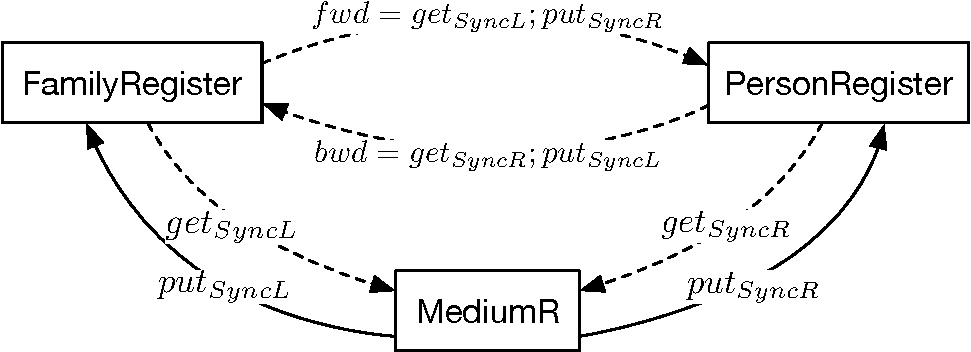
\includegraphics[width=\columnwidth]{diagrams/solutions/bigulSolnOverview}
    \caption{Handling a symmetric bx with BiGUL}
    \label{fig:bigulSolnOverview}
\end{figure}
%
In this decomposition, an additional data structure \texttt{MediumR} is introduced and can be thought of intuitively as the intersection of both data structures, i.e., it contains exactly the concepts that are present in both the source and target model spaces and that must be kept consistent.
All the bx developer now has to do is program how \texttt{MediumR} models can be \emph{put} into \texttt{Person\-Regis\-ter} models via $put_{SyncR}$, and into \texttt{Family\-Regis\-ter} models via $put_{SyncL}$.
The required \emph{fwd} and \emph{bwd} transformations can now be computed as depicted in figure~\ref{fig:bigulSolnOverview} by composing programmed \emph{put} and derived \emph{get} arrows as required.\footnote{The actual solution is a bit more complex as \emph{SyncL} is further decomposed into two arrows.}

To provide some details for actual BiGUL code, figure~\ref{fig:bigulSolnDetails} depicts the BiGUL program for $put_{SyncR}$.
Recall that the architecture for this solution is restoration-based (with $hAln$) for an initial-state-based scenario.
So this code conceptually represents \emph{fCR} and $hAln$ (see figure~\ref{fig:initialStateBased}).
The parts of the code representing $hAln$ are in black with a white background, while parts representing \emph{fCR} are in white with a black background.

\begin{figure}[tbp]
    \centering
    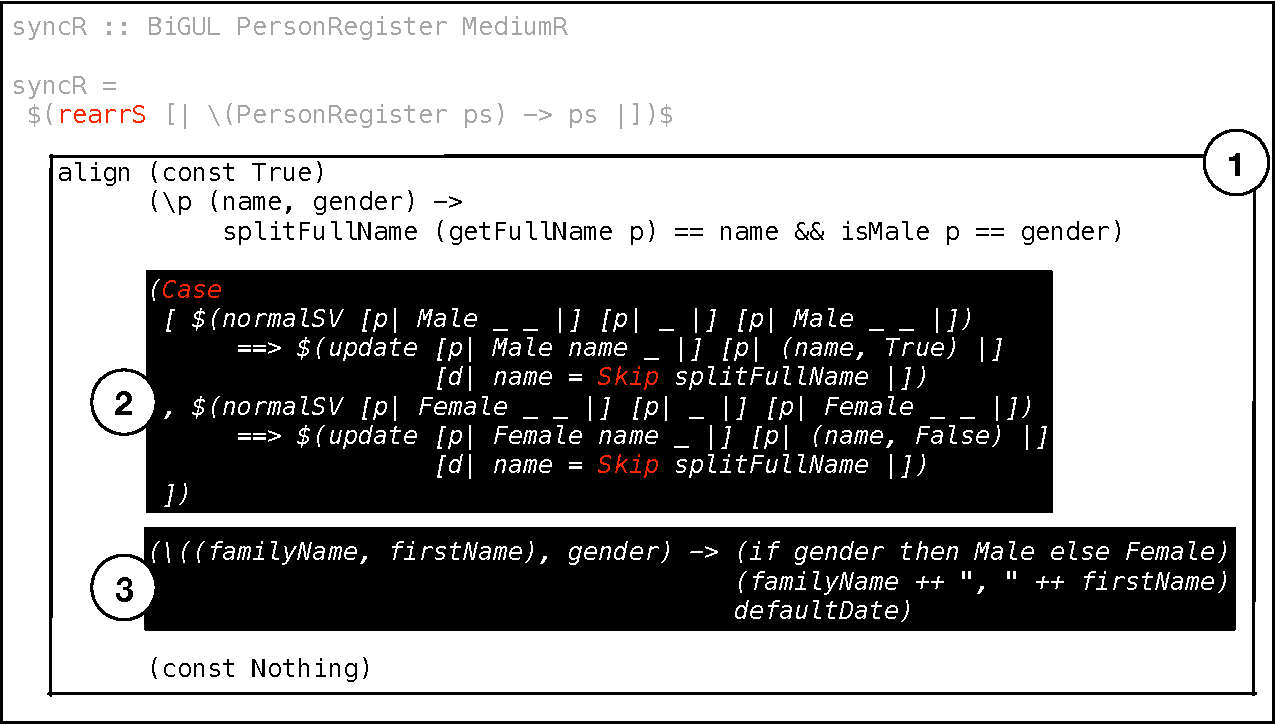
\includegraphics[width=\columnwidth]{diagrams/solutions/bigulSolnDetails}
    \caption{Structure of a BiGUL program}
    \label{fig:bigulSolnDetails}
\end{figure}

As both models are essentially lists (of persons and $(name, gender)$ pairs) $hAln$ can be implemented with the auxiliary function \texttt{align} that takes a matching condition and uses it to lift a BiGUL program on elements to lists (marked with label 1 in figure~\ref{fig:bigulSolnDetails}).
The simple strategy is to traverse the list of view elements and to search for the first source element that matches according to the condition (here simply a comparison of name and gender).
If a match is found then the first part of the \emph{fCR} code (label 2) is executed (it does nothing as the elements are already consistent), if no match can be found then a new source element is created using the second part of the \emph{fCR} code (label 3).
If unmatched source elements remain after all view elements have been matched, they are simply deleted by \texttt{align}.

Finally, although the code might appear cryptic without looking up all details, the used BiGUL primitives are highlighted red in figure~\ref{fig:bigulSolnDetails}.
The point here is that the entire program is a composition of primitives, designed in a way that this resembles programming in a standard (imperative) programming language.


\subsection{BXtend}
\label{sec:BXtend}

\NOTE{\emph{Solution expert:} Thomas, \emph{Interviewer:} Tony}

Classification according to our feature model:

style:  restoration-based
application scenario:  initial-diag-based
well-behavedness guarantees: none
consistency relation: implicit
synchronization: on-demand, explicit control

Extra details concerning architecture:

Applies restoration-based architecture depicted in figure~\ref{fig:initialDiagBased}.
\emph{fCR/bCR} is decomposed into multiple ``rules'' consisting of restoration logic separated into forward and backward direction.
Each rule defines flexibly, e.g., based on a certain type, if it is applicable or not.
Similarly, each rule checks first by exploiting the supplied corr if existing structure in the dependent model can be reused, suitably changed, or deleted and created as required.
To perform \emph{fCR/bCR} an orchestration component is supplied to decide the order in which individual rules are applied and combined to realize \emph{fCR/bCR}.
This global component can also perform a final clean up if this is required.
The delta created as output is mixed in the sense that each rule can already perform deletion and creation as required.

Technical, language-related points:

Xtend is used as implementation language to provide a compact, readable syntax.
As Xtend integrates seamlessly with Java, Java can also be used in the implementation.

Conclusion:

+ flexible, solutions can be made very efficient, full control over the synchronization process, low learning curve

- no guarantees, solutions can be just as inefficient if preconditions of rules are costly to check (as this is checked for the entire model) => a bad programmer can produce unreadable, inefficient, and incompatible \emph{fCR/bCR}.

\subsection{eMoflon}
\label{sec:eMoflon}

\NOTE{\emph{Solution expert:} Tony, \emph{Interviewer:} Zinovy}

TODO

\subsection{EVL+STrace}
\label{sec:EVLPlusSTrace}

\NOTE{\emph{Solution expert:} Leila , \emph{Interviewer:} Thomas}

\subsection{JTL}
\label{sec:JTL}

\NOTE{\emph{Solution expert:} Romina, \emph{Interviewer:} Tony}

TODO

%\clearpage

\subsection{NMF Synchronizations}
\label{sec:NMF}

\NOTE{\emph{Solution expert:} Georg, \emph{Interviewer:} Bernhard}

\subsubsection{Approach}
\label{sec:ApproachNMF}

NMF Synchronizations \cite{SoSyM2017-Hinkel}is a bx language which is formally based on category theory. Consistency between two models is defined in terms of consistency relations between their elements. In the case of mutual consistency, an element-level consistency relation is an \emph{isomorphism} between typed source and target elements, i.e., a bijective mapping between elements of some type $A$ in the source model and elements of some type $C$ in the target model satisfying specified consistency constraints. Consistency relations are coupled: For an $A$-element to be consistent with a $C$-element, an isomorphism between dependent source and target elements (of types $B$ and $D$)may be required. In addition to defining element-level consistency relations, consistency restoration has to be specified, provided that no default restoration is available.

\begin{figure}[tb!]
	\centering
	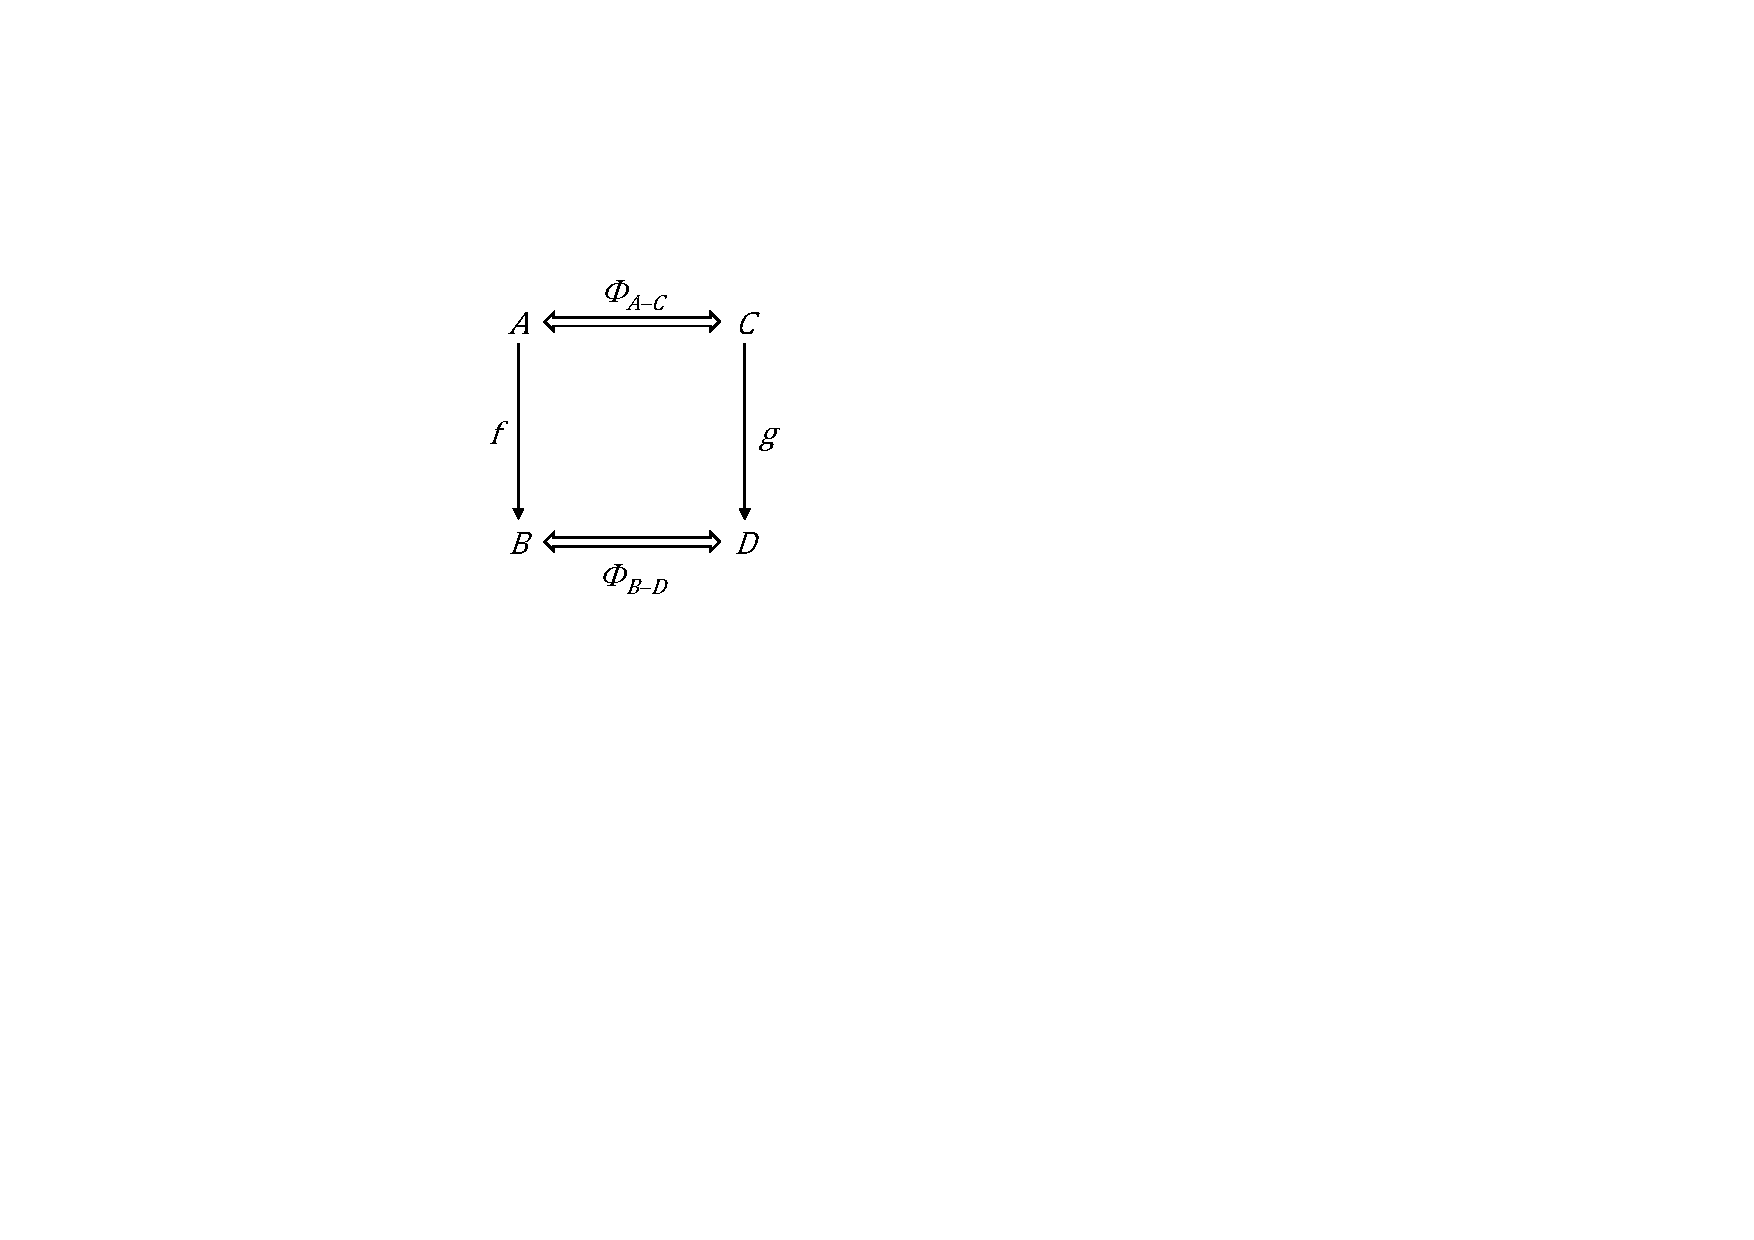
\includegraphics[width=0.35\columnwidth]{diagrams/NMFSynchronizationBlock}
	\caption{Schematic view of a synchronization block}
	\label{fig:SynchronizationBlock}
\end{figure}

The overall synchronization is specified in terms of \emph{synchronization blocks}, which are illustrated schematically in Figure~\ref{fig:SynchronizationBlock}. The isomorphisms mentioned above are represented by horizontal arrows. The isomorphism $\varPhi_{A-C}$ on the top is called \emph{base isomorphism}, while $\varPhi_{B-D}$ at the bottom plays the role of the \emph{target isomorphism}. A target isomorphism may occur as base isomorphism in another synchronization block, resulting in nested synchronization blocks. Furthermore, an isomorphism may play the role of a base isomorphism in multiple synchronization blocks, meaning that multiple consistency relations are required for making a pair of elements in the base isomorphism consistent.

The vertical arrows labeled with $f$ and $g$ denote \emph{intra-model lenses}. An intra-model lense is composed of a pair of functions called \emph{Get} and \emph{Put}. \emph{Get} and \emph{Put} are queries and updates on model elements --- in the simplest case getters and setters of element properties --- which have to satisfy round-trip laws: (1) Putting the result returned from a \emph{Get} does not change the state of the model; (2) Getting a value after a \emph{Put} returns the argument passed to the \emph{Put} operation.

Depending on the results returned from \emph{Get} operations, synchronization blocks may be classified into single-and multi-valued blocks. In the case of a \emph{single-valued block}, the \emph{Get} functions return single values which have to be consistent (e.g., the values are required to be equal). For a \emph{multi-valued block}, the \emph{Get} functions return collections. In this case, an isomorphism between these collections must be established.

The consistency relation between two models is defined by the synchronization blocks, using only the \emph{Get} operations. For consistency restoration, the \emph{Put} operations, are required, as well. For example, in a forward transformation the \emph{Get} operations on the source model are needed to retrieve the source model elements with which consistency has to be established in the target model. For updating the target model, the corresponding \emph{Put} operations are required. In simple situations, a \emph{Put} operation may be derived from the \emph{Get} operation. Otherwise, the transformation developer has to provide an explicit specification of \emph{Put} satisfying the round-trip laws of intra-model lenses. 

Altogether, the transformation developer defines the consistency relation declaratively in a functional style with the help of synchronization blocks and their \emph{Get} operations. This specification is complemented with the provision of \emph{Put} operations, which are written in a procedural style. A single specification suffices to define mutual consistency; in this regard, NMF Synchronizations is a bidirectional language. This specification is complemented with unidirectional procedural parts defining how consistency is restored in forward and backward direction, respectively.

\subsubsection{Solution}
\label{sec:solutionNMF}

NMF Synchronization is an \emph{internal DSL} based on the host language C\#. The following description is based on the solution in NMF Synchronizations submitted to TTC 2017 \cite{Hinkel2017}. Listing~\ref{lst:nmf} shows fragments of this solution, to be explained below. Since NMF Synchronization is a part of \emph{NMF} \cite{Hinkel2016}, the .NET Modeling Framework, the solution to the Families to Persons benchmark runs in a separate process which communicates with the EMF-based Benchmarx process via data streams. Below, we will not explain how this coupling is implemented; rather, we will focus on the actual core solution.



\lstdefinelanguage{cs}{
	morekeywords = {using,namespace,class,override,void,null,public,protected,private,static,out,bool,string,return,var,new,true,false,if,else,as},
	morecomment=[l]{--},
	morecomment=[s]{/*}{*/}
}


\begin{lstlisting}[label={lst:nmf}, float=*t, language=cs, caption={Solution in NMF Synchronizations}]
namespace TTC2017.FamiliesToPersons.NMF {
    public class FamiliesToPersonsSynchronization : ReflectiveSynchronization {
        public class FamilyRegisterToPersonRegister : SynchronizationRule<FamilyRegister, PersonRegister> {
            public override void DeclareSynchronization() {
                SynchronizeMany(SyncRule<MemberToMember>(),
                    fam => new FamilyMemberCollection(fam),
                    persons => persons.Persons);
            }
        }

        public class MemberToMember : SynchronizationRule<IFamilyMember, IPerson> {
            public override void DeclareSynchronization() {
                Synchronize(m => m.GetFullName(), p => p.Name);
            }
        }
        
        public class MemberToFemale : SynchronizationRule<IFamilyMember, IFemale> {
            public override void DeclareSynchronization() {
                MarkInstantiatingFor(SyncRule<MemberToMember>(), 
                    leftPredicate: m => m.MotherInverse != null || m.DaughtersInverse != null);
            }
            ...
        }
        
        private class FamilyMemberCollection : CustomCollection<IFamilyMember> {
            ...
            public override void Add(IFamilyMember item) {
                var temp = item.GetExtension<TemporaryStereotype>();
                item.AddToFamily(Register, temp.IsMale, temp.LastName);
                item.Extensions.Remove(temp);
            }
            ...
        }
        ...
    }
}
\end{lstlisting} 

In NMF Synchronizations, a transformation is defined by extending classes from a library. In Listing~\ref{lst:nmf}, the overall transformation is defined by a single top-level class (starting at line~2) containing further nested classes.

A \emph{synchronization rule} includes all synchronization blocks sharing the same base isomorphism. In the Families to Persons benchmark, each synchronization rule contains just one synchronization block. A synchronization rule is defined by subclassing the generic class \code{SynchronizationRule} (lines~3, 11, and 17). This class is equipped with two generic parameters for the types of the source and the target elements of the base isomorphism, respectively. The actual synchronization blocks are defined by overriding the method \code{Declare\-Synchron\-ization} (lines~4, 12, and 18). 

Altogether, the class starting at line~3 defines a multi-valued synchronization block with a base isomorphism between the roots of the families model and the persons model (of type \code{FamilyRegister} and \code{Person\-Register}, respectively) and a target isomorphism between family members and persons. The call to the method \code{SynchronizeMany} specifies the nested synchronization rule \code{MemberToMember}, as well as the \emph{Get} functions for retrieving the collections of family members and persons as Lambda expressions. 

\code{persons.Persons} is an \emph{invertible expression}: Since the \emph{Get} function merely collects the elements obtained via a multi-valued reference, the updates may be inferred automatically. In contrast, a \emph{custom collection} is required at the opposite end, which is implemented in the helper class \code{FamilyMemberCollection} (line~25). The implementation of the helper class has to define the path for getting the elements of the collection (traversing references to families and members sequentially), which is not shown here, and has to provide an update method for adding a family member to the collection (line~27). This \code{Add} method is required in a backward transformation to insert an already created family member at the appropriate location into the families model. To this end, a custom method \code{AddToFamily} is called (line~29) which performs this insertion depending on the configuration parameters \code{PreferExistingToNew\-Family} and \code{PreferParentToChild}. The information on the gender and the last name of the family member is retrieved from temporary stereotypes attached to the model element (line~28); these stereotypes are removed in line~30.

\code{MemberToMember} defines a single-valued synchronization block which demands that the full name of the family member be synchronized with the name of the person (i.e., the respective strings must be equal). The method \code{GetFullName} composes the full name from the first name and the last name in a straightforward way. In addition to this \emph{Get} function, we need to supply the corresponding \emph{Put} to complete the definition of the intra-model lense. To this end, a custom method \code{SetFullName} is defined which sets the full name, potentially moving the member to a different family (both methods are not shown due to the lack of space).

Finally, we need to take care of the fact that the class \code{Person} is abstract and thus cannot be instantiated in forward direction. This is achieved by two synchronization rules, one of which is shown in line~17. The rule \code{MemberToFemale} refines the rule \code{MemberToMember} by defining the type to be instantiated. Please note that the base isomorphism of the synchronization is refined to \code{IFemale} on the persons model. Furthermore, the method call in line~19 defines the predicate which has to be satisfied in order to apply this refinement (the member must be a mother or a daughter).  




\begin{figure*}[htb!]
	\centering
	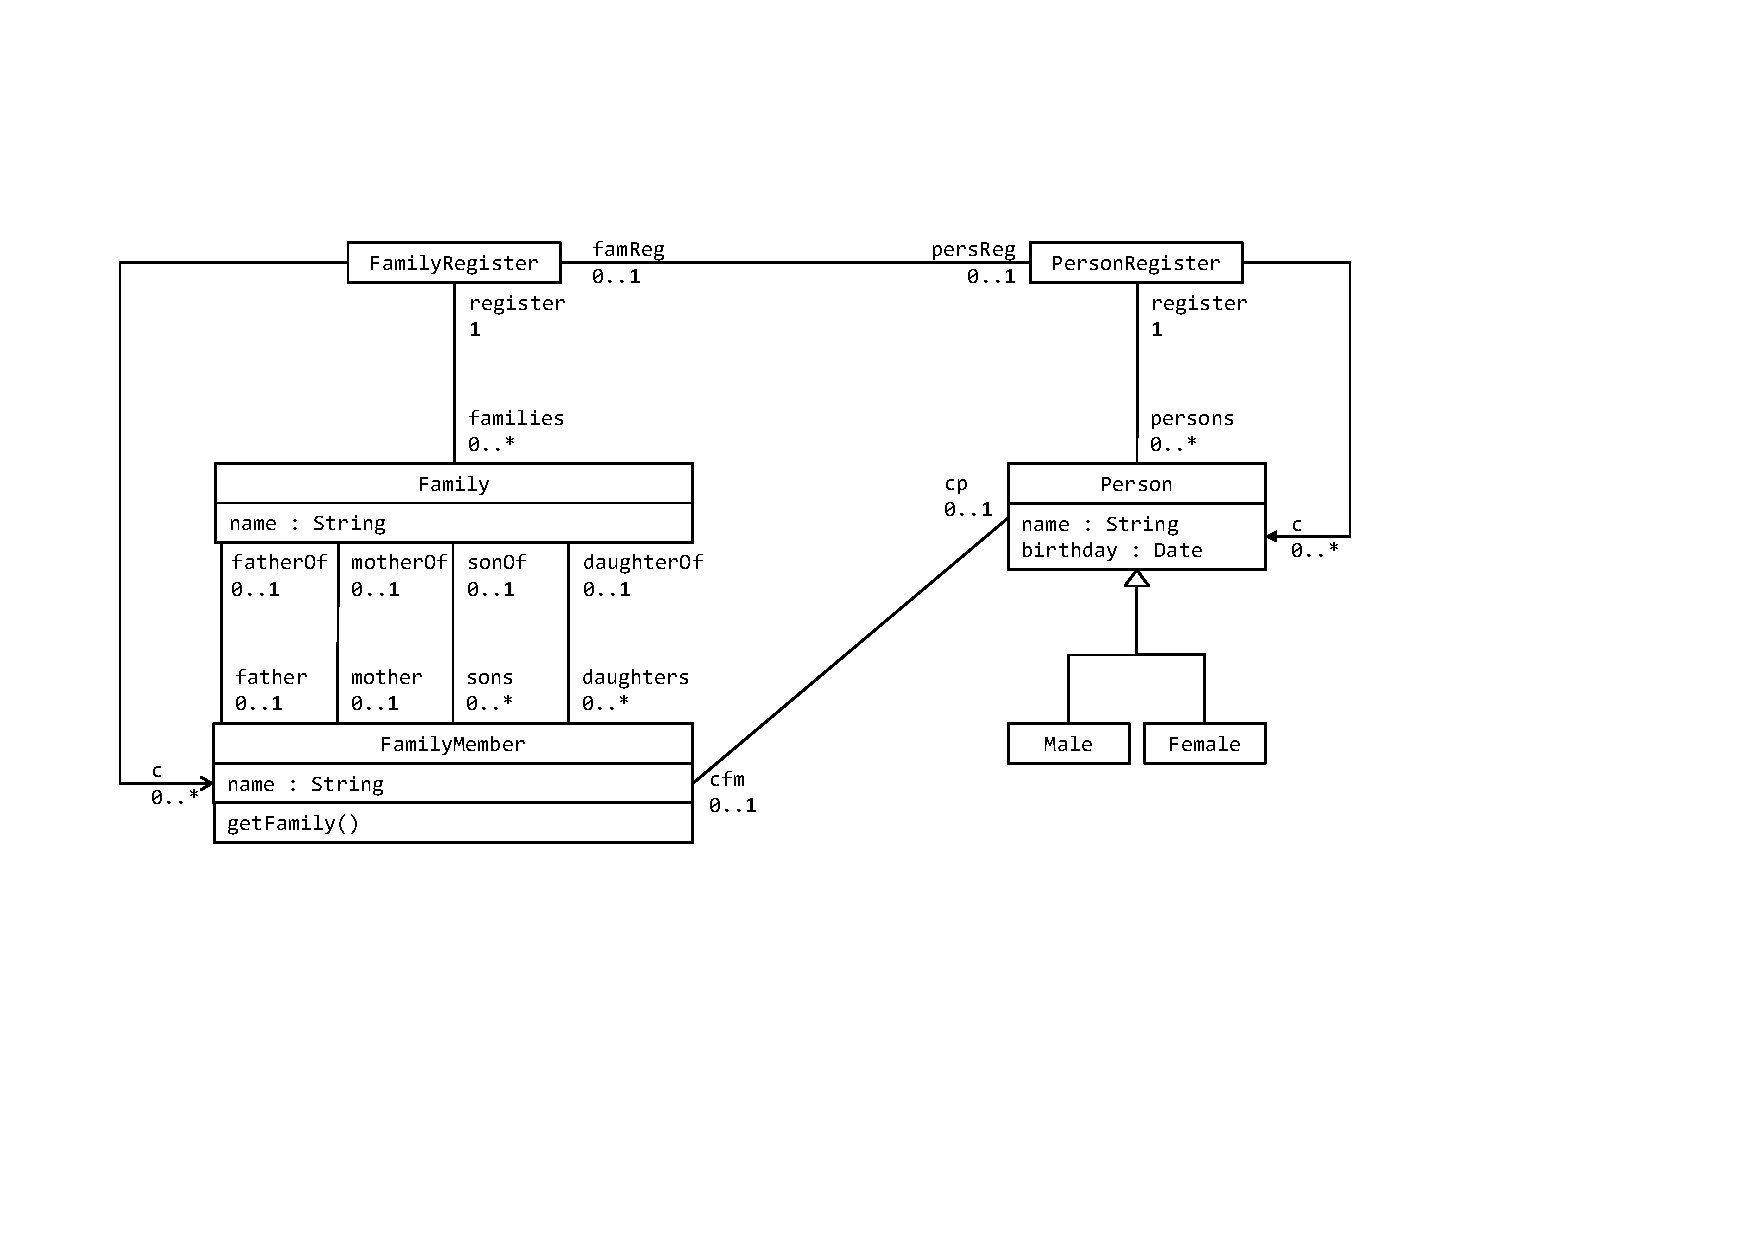
\includegraphics[width=0.75\textwidth]{diagrams/solutions/SDMLibModel}
	\caption{SDMLib model used for the benchmark}
	\label{fig:SDMLibModel}
\end{figure*}

\subsection{SDMLib}
\label{sec:SDMLib}

SDMLib, short for \emph{Story Driven Modeling Library}\footnote{http://www.sdmlib.org}, is a Java library to support Story Driven Modeling~\cite{Norbisrath2013}, a formalism based on graph transformations~\cite{Ehrig2006}.
SDMLib provides an internal DSL with Java as a host language.
Although SDMLib is not a bx tool, in the sense that it does not provide any extra support especially for developing bx, it is nonetheless included here as a ``general purpose'' model transformation tool against which bx tools should also be compared. 

As models can be viewed as attributed, typed \emph{graphs}, model transformations can also be regarded as a problem in the domain of graph transformations.
A \emph{graph rewrite rule} specifies the replacement of a graph pattern (left-hand side) by a subgraph to be embedded into the overall host graph.
Graph rewrite rules can be used to specify not only in-place model transformations, but also 
model-to-model transformations by applying the rules to multiple graphs.
Graph rewrite rules are \emph{declarative} in the sense that the exact order in which to traverse the host graph and check for or replace patterns is not specified.


\subsubsection{Classification}
The solution to the benchmark with SDMLib follows a \emph{restoration-based} architectural style; \emph{fCR} and \emph{bCR} are implemented with graph rewrite rules. 

The solution addresses the \emph{initial-diag-based} application scenario (figure \ref{fig:initialDiagBased}).
A diag is taken as input, and the dependent model is manipulated until both models are consistent again. 

No formal guarantees are provided by SDMLib as \emph{fCR} and \emph{bCR} are specified separately and independently.
It is left up to the transformation developer to ensure that the implementations are not contradictory.
As with the BXtend solution, this can be viewed as an advantage; the bx programmer may freely decide whatever is necessary to solve the current task.

The SDMLib solution has no explicit notion of \emph{consistency} as it is \emph{implicitly} given by the implemented pair of \emph{fCR/bCR}.
Accordingly, synchronization \emph{control} is \emph{explicit}, and programmed by providing suitable graph rewrite rules.
The SDMLib solution was developed with the benchmark in mind and thus supports \emph{directed}, \emph{on demand}, \emph{automatic} synchronization. 

\subsubsection{Benchmark solution with SDMLib}

The following description is based on the SDMLib solution for the Families-to-Persons benchmark at TTC 2017~\cite{Zundorf2017}.
As SDMLib is designed for in-place transformations on a single host graph, the solution uses a single metamodel as depicted in figure~\ref{fig:SDMLibModel}.
To support incrementality efficiently, additional unidirectional references between \code{FamilyRegister} and \code{Fami\-lyMember}, and \code{PersonRegister} and \code{Person} are used to detect changed elements.
Finally, the correspondences are represented using two bidirectional references.
The SDMLib solution thus operates on a single graph comprising the contents of both models as well as explicit correspondence links between respective elements. 

\begin{lstlisting}[label={lst:sdmlib}, float=hbt!, language=java, caption={Forward transformation in SDMLib}]
private void transformForward() {
 familyRegisterPO = new FamilyRegisterPO()
   .withPatternObjectName("fr");
 PersonRegisterPO personRegisterPO = 
  familyRegisterPO.createPersonRegisterPO()
                  .withPatternObjectName("pr");
 FamilyMemberPO memberPO = familyRegisterPO
   .createCPO()
   .withPatternObjectName("fm");

 // there is an old corresponding person
 memberPO.startSubPattern();
 PersonPO oldPersonPO = memberPO.createCpPO()
   .withName("oldP");
 oldPersonPO.createCondition(p -> 
   ensureNameAndGender(p));
 memberPO.endSubPattern();

 // no corresponding person
 memberPO.startNAC();
 memberPO.createCpPO()
   .withPatternObjectName("noOldP");
 memberPO.endNAC();
 MalePO personPO = memberPO
   .createCpMalePO(Pattern.CREATE)
   .withPatternObjectName("newP");
 personPO.createRegisterLink(
   personRegisterPO, 
   Pattern.CREATE);
 personPO.createCondition(p -> 
   ensureNameAndGender(p));
    
 familyRegisterPO.createLink(
   memberPO, 
   Pattern.DESTROY);

 familyRegisterPO.rebind(familyRegister);
 familyRegisterPO.doAllMatches();	    
}
\end{lstlisting}

The core of the SDMLib solution consists of two graph rewrite rules, one for each direction.
While graph rewrite rules are typically presented using a visual concrete syntax, we use the actual textual concrete syntax provided by the tool to enable and simplify a comparison with all other solutions.  

Listing~\ref{lst:sdmlib} depicts the graph rewrite rule for the forward transformation using SDMLib's internal DSL, embedded into Java.
The method for the graph rewrite rule uses code generated from the graph metamodel depicted in figure~\ref{fig:SDMLibModel}. 

The statements on line~2--9 define story pattern objects for the family register, the person register, and a family member, which need to be matched in the families model; the links connecting these objects are added implicitly to the story pattern by the invoked methods (e.g., \code{createCPO()}). 

Lines~12-17 handle the case that a corresponding person object already exists.
This case is realized with an optional subpattern, which is started at line~12 and is terminated at line~17.
The pattern is composed of an old person object, connected to the family member object by a correspondence link.
If pattern matching succeeds, the method \code{ensure\-Name\-And\-Gender} is invoked to restore consistency.

Lines~20--31 deal with the case where there is no corresponding person object.
This is handled with a \emph{negative application condition}, defined on lines~20--23.
On lines~17--19, elements of story patterns are created that define the actions to be performed when the negative application condition holds: A person object has to be created and linked to the person register; the method \code{ensure\-Name\-And\-Gender} is then called to establish consistency with the family object.

Finally, the temporary link between the family register and the family member --- which is set in the course of changes to the families model --- is matched and then removed (lines~33--35), the story pattern object for the family register is bound (line~37), and the pattern is applied to all matches (line~38).

%%% Local Variables:
%%% mode: latex
%%% TeX-master: "../main"
%%% End:


%%% Local Variables:
%%% mode: latex
%%% TeX-master: "../main"
%%% End:


\section{Evaluation}
\label{sec:Evaluation}

\NOTE{Focus on properties which can be measured, leave out others (level of abstraction, cognitive complexity).}

After having presented solutions for the Families-to\-Persons benchmark, we will now address their evaluation with respect to three measurable properties: size of the transformation definition, measured in terms of lines of code; correctness, measured in terms of passed and failed test cases; performance, measured in terms of runtime. We will leave out other properties such as level of abstraction or cognitive complexity, which are relevant, but difficult to measure. Beforehand, we will state some hypotheses concerning expected results, which will be revisited after having presented the actual evaluation results. We will conclude with some remarks on threats to validity.

\subsection{Hypotheses}
\label{sec:Hypotheses}

Before presenting the actual evaluation of the solutions for the Families-to-Persons case, we state some hypotheses concerning the expected results. These hypotheses are based on the features of bx tools, as introduced in section~\ref{sec:Foundations} and summarized in figure~\ref{fig:featureModelBxTools}, and are exemplified with the help of the classification of the bx tools in which the benchmark case was solved (table~\ref{tab:features-all-tools}). We will revisit our hypotheses after having presented the results of our evaluation, and discuss to what extent they are supported by the evaluation results. 

\subsubsection{Size of transformation definitions}
\label{sec:HypothesesSize}

\begin{hypothesis}
	\label{hyp:size1}
	Implicit control reduces the size of a transformation definition.
\end{hypothesis}

\emph{Justification.} In the case of implicit control, there is no need to program synchronization behavior explicitly; rather, it is derived from some specification. Either the consistency relation is specified (e.g., in terms of constraints as in JTL or grammar rules as in eMoflon), or one direction of the synchronization is derived from the opposite, explicitly programmed direction (BiGUL). In any case, it is expected that the size of a transformation definition is reduced because there is no need to program both directions of synchronizations explicitly. 

\subsubsection{Correctness}
\label{sec:HypothesesCorrectness}

A solution is considered \emph{correct} if it satisfies the requested execution behavior. As far as the benchmark is concerned, a solution is considered correct if it passed all test cases. 

\begin{hypothesis}
	\label{hyp:correctness1}
	Implicit control trades expressiveness\\for well-behavedness guarantees.
\end{hypothesis}

\emph{Justification.} Approaches which are based on implicit control provide certain well-behavedness guarantees at the cost of expressiveness. I.e., these guarantees are given only under certain assumptions: In BiGUL, round-trip laws hold only when transformations are composed from a restricted set of primitives, in eMoflon restrictions apply to grammar rules, etc. Thus, the class of bidirectional transformations which may be expressed in approaches based on implicit control is usually restricted. As a consequence, it may not be possible to fully realize the requested synchronization behavior.

\begin{hypothesis}
	\label{hyp:corrrectness2}
	The ability to achieve correctness increases with the amount of input data used by a bx tool.
\end{hypothesis}

\emph{Justification.} The application scenario (figure~\ref{fig:featureModelBxTools}) strongly determines the capabilities of a bx tool. At the low end of the spectrum, an initial-state-based tool like BiGUL merely receives the new version of the master model and the old version of the dependent model as inputs. At the opposite high end, an o-delta-corr-based tool like NMF may exploit correspondences between models which may not be reconstructable based on the model states alone. Furthermore, it may precisely propagate operational deltas, processing the operations in the order in which they were executed, and may thus realize order-dependent synchronization. 

\subsubsection{Performance}
\label{sec:HypothesesPerformance}

\begin{hypothesis}
	\label{hyp:performance}
	Delta-based synchronization increases\\the performance of incremental synchronizers.
\end{hypothesis}

\emph{Justification.} A bx tool such as eMoflon or NMF which receives a (structural or operational) delta as input is provided with the information which change operations have been applied at which locations. This knowledge may be exploited to restore consistency efficiently. In contrast, bx tools which lack this information (e.g., BiGUL or BXtend) need to perform a global analysis to derive the delta. This analysis may be expensive in the case of large models; the cost of restoring consistency may be neglectable compared to the cost of analysis.  

\subsection{Test Suite}
\label{sec:TestSuite}

\NOTE{\emph{Length:} 1 p., \emph{Responsible:} Thomas}

\NOTE{Design of the internal DSL, package structure of test cases, classification of test cases according to the taxonomy}

\renewcommand{\arraystretch}{1.2}

%\newcolumntype{P}[1]{>{\centering\arraybackslash}p{#1}}
%\newcolumntype{M}[1]{>{\centering\arraybackslash}m{#1}}
\begin{table*}[!tbp]
	\begin{tabular}{M{7cm}|M{1.4cm}|M{1.6cm}|M{1.9cm}|M{1.3cm}|M{1.3cm}}
		\textbf{Name of Test} & \textbf{Direction} & \textbf{Horizontal Input} & \textbf{Vertical Input} & \textbf{Change Type} & \textbf{Runtime Config}  \\ \hline
		\textit{testInitialiseSynchronisation} & fwd/bwd & none & initial-based & - & no   \\ \hline
		\textit{testFamilyNameChangeOfEmpty} & fwd & none & initial-based & attribute  & no \\ \hline
		\textit{testCreateFamily} & fwd & none & initial-based & add & no \\ \hline
		\textit{testCreateFamilyMember} & fwd & none & initial-based & add & no \\ \hline
		\textit{testDuplicateFamilyMemberNames} & fwd & none & initial-based & add & no \\ \hline
		\textit{testNewDuplicateFamilyNames} & fwd & none & initial-based & add & no \\ \hline
		\textit{testNewFamilyWithMultiMembers} & fwd & none & initial-based & add & no \\ \hline
		\textit{testCreateFamilyMembersInExistingFamily\-As\-Parent} & bwd & none & initial-based & add & yes \\ \hline
		\textit{testCreateMalePersonAsSon} & bwd & none & initial-based & add & yes \\ \hline
		\textit{testCreateFamilyMemberInExistingFamily\-As\-Children} & bwd & none & initial-based & add & yes \\ \hline
		\textit{testCreateDuplicateFamilyMembersInExisting\-Family\-As\-Children} & bwd & none & initial-based & add & yes \\ \hline
		\textit{testCreateMalePersonAsParent} & bwd & none & initial-based & add & yes \\ \hline
		\textit{testCreateFamilyMembersInNewFamily\-As\-Parents} & bwd & none & initial-based & add & yes \\ \hline
		\textit{testCreateDuplicateFamilyMembersInNewFamily\-As\-Parents} & bwd & none & initial-based & add & yes \\ \hline
		\textit{testCreateFamilyMembersInNewFamily\-As\-Children} & bwd & none & initial-based & add & yes \\ \hline
		\textit{testCreateDuplicateFamilyMembersInNewFamily\-As\-Children} & bwd & none & initial-based & add & yes \\ \hline
		\textit{testIncrementalInserts} & fwd & state-based & state-based & add & no\\ \hline
		\textit{testIncrementalDeletions} & fwd & corr-based & s-delta-based & del & no \\ \hline
		\textit{testIncrementalRename} & fwd & corr-based & s-delta-based & attribute & no \\ \hline
		\textit{testIncrementalMove} & fwd & state-based & s-delta-based & move (del+add) & no \\ \hline
		\textit{testIncrementalMixed} & fwd & state-based & s-delta-based & add, del & no \\ \hline
		\textit{testIncrementalRoleChange} & fwd & state-based & s-delta-based & add, del & no\\ \hline
		\textit{testStability} & fwd & state-based & state-based & - & no \\ \hline
		\textit{testHippocraticness} & fwd & state-based & state-based & attribute & no\\ \hline
		\textit{testIncrementalInsertsFixedConfig} & bwd & state-based & state-based & add & yes \\ \hline
		\textit{testIncrementalInsertsDynamicConfig} & bwd & state-based & state-based & add & yes \\ \hline
		\textit{testIncrementalDeletions} & bwd & state-based & state-based & del & yes \\ \hline
		\textit{testIncrementalRenamingDynamic} & bwd & corr-based & s-delta-based & attribute & yes \\ \hline
		\textit{testIncrementalMixedDynamic} & bwd & state-based & s-delta-based & add, del & yes \\ \hline
		\textit{testIncrementalOperational} & bwd & state-based & o-delta-based & add & yes \\ \hline
		\textit{testStability} & bwd & state-based & state-based & - & yes \\ \hline
		\textit{Hippocraticness} & bwd & state-based & state-based & attribute & yes \\ \hline
	\end{tabular}
	\caption{Classification of Test Cases according to the Taxonomy}
	\label{tab:classification-test-cases}
\end{table*}

\subsection{Size of transformation definitions}
\label{sec:Size}

\NOTE{\emph{Length:} 0.5 p., \emph{Responsible:} Thomas}

\NOTE{In lines of code and/or number of tokens?}

A quantitative evaluation of the different tools and solution to the Families-to-Persons case presented in this paper may be given by comparing the size of the dif\-ferent transformation definitions. As all of the discussed solutions are based on tools allowing for a textual specification of model-transformations, a comparison in terms of the following metrics is provided:
\begin{description}
	\item[Lines of Code:] The total number of source code lines needed to describe the transformation. Empty lines as well as lines containing comments are not considered in this metrics.
	\item[Number of Words:] The total number of words used in the transformation specification (comments are ignored).
	\item[Number of Characters:] The total number of characters used for the Families-to-Persons transformation (comments are omitted).
\end{description}

\renewcommand{\arraystretch}{1.2}

\newcolumntype{P}[1]{>{\centering\arraybackslash}p{#1}}
\newcolumntype{M}[1]{>{\centering\arraybackslash}m{#1}}
\begin{table*}[!tbp]
	\begin{tabular}{M{1.55cm}|M{1.7cm}|M{1.6cm}|M{1.9cm}|M{2.1cm}|M{1.7cm}|M{1.7cm}|M{1.5cm}}
		\textit{} & \textbf{BiGUL} & \textbf{BXtend} & \textbf{eMoflon} & \textbf{EVL+STrace} & \textbf{JTL} & \textbf{NMF} & \textbf{SDMLib} \\ \hline
		\textit{Lines of Code} & 176 & 211 & 192 & 1299 & 168 & 279 &  236 \\ \hline
\textit{Number of Words} & 1010 & 565 & 256 & 2878 & 260 & 607 &  427 \\ \hline
\textit{Number of Characters} & 6197 & 7571 & 3195 & 50109 & 4338 & 7215 &  6761 \\ \hline

	\end{tabular}
	\caption{Size of the transformation definitions of all tools and solutions}
	\label{tab:size-all-solutions}
\end{table*}

Table \ref{tab:size-all-solutions} shows the numbers obtained for the metrics described above. They give a good impression about the effort required to specify the transformation as well as the verbosity of the used tools. Hypothesis 1 (see Section \ref{sec:HypothesesSize}) implies that declarative approaches, which allow for the derivation of both transformation directions from a single specification should require significantly smaller transformation definitions. JTL, BiGUL and eMoflon are tools that allow specifications on a high level of abstraction and an explicit programming of the synchronization behavior is not required. As a result the corresponding transformation specifications are the smallest in this comparison. However, for resolving non-determinism in the backward direction, additional code was required for eMoflon and JTL. While in eMoflon Java code was supplied to orchestrate the code generated from the TGG specification, a significant amount of ASP code was needed for JTL. \NOTE{Tony, could you please supply the missing numbers?}
The most interesting observation is that both BXtend and SDMLib almost match the size of the JTL, eMoflon and BiGUL specifications although in both tools each transformation specification has to be programmed explicitly. The EVL+Strace specification requires approx. 7 times as much lines of code as the most concise specification. 

\subsection{Correctness}
\label{sec:Correctness}

\NOTE{\emph{Length: 2 p.}, \emph{Responsible:} Tony and Thomas for global table, solution experts for tool specific paragraphs.}

\NOTE{Table of failed and solved test cases. Distinguish between pass and fail, expected and unexpected. Discuss each tool in one paragraph.}

\subsection{Performance}
\label{sec:Performance}

\NOTE{\emph{Length:} 1 p., \emph{Responsible:} Tony}

\NOTE{Debatable whether and to what extent this should be included. Maybe only partial results could be presented here.}

\subsection{Hypotheses revisited}
\label{sec:HypothesesRevisited}

\subsection{Threats to validity}
\label{sec:ThreatsToValidity}

\NOTE{\emph{Length:} 0.5 p., \emph{Responsible:} Tony, Thomas}

Threat:  Our collection of tests is ad-hoc, i.e., we did not "cover" the feature model in any systematic manner.  This could be improved in the future using combinatoric approaches such as all pairs of features, etc.   

Mitigation:  We discussed the tests (three researchers using 3 different tools) and decided together what is correct and incorrect (at least not just one person).  Tests were again discussed during TTC with feedback/review from solution experts.  Test suite is not meant to be complete in any sense and is only to demonstrate what is possible with the framework.

Measurements:  

EMF compatibility:
- NMF requires costly conversion so we had to omit this when measuring (also the reason why we had to extrapolate values)
- BiGUL also required conversion but this was negligible so we did not do any handling
- SDMLib uses a rewrite of the tests to solve the compatibility problem
- all other tools are EMF conform and could work directly with the models
- weren't able to automate EVL+STrace as required (rather slow though based on manual tests)

Non-determinism, manual steps:

- EVL+STrace required a series of complex manual steps.  This means that the probability of making manual errors is also higher.

- eMoflon (pattern matching) is non-deterministic.  Some tests might fail if repeated often enough.

Just a single, rather simple example

Plots might be different for different deltas (wrt. incremental updates)

Framework:

- Threat: is clearly delta-based and favours corr-based, delta-based approaches. 
- Mitigation:  Interpretation of test results and classification in expected/unexpected fails/passes.  This enable a fair evaluation of tools with a restricted set of features.



\section{Related Work}
\label{sec:RelatedWork}

\NOTE{\emph{Length:} 1 p., \emph{Responsible:} Bernhard}

\NOTE{Mandatory part of a journal paper. At least, relations to previous publications of the main authors have to be established. Work of others on benchmarking bidirectional transformations? Work on classification, e.g., SoSyM paper by Hidaka?}

\subsection{Benchmark frameworks}
\label{sec:BenchmarkFrameworks}

To the best of our knowledge, Benchmarx is the first and only framework for developing and executing benchmarks for bidirectional transformations. The framework is based on initial conceptual work regarding the requirements which bx benchmarks and benchmark frameworks should satisfy \cite{AnjorinCG0RS14}. An implementation of these concepts was developed several years later and described in a paper for the BX 2017 workshop \cite{Anjorin2017}. This article goes considerably beyond the workshop paper inasmuch as it presents the selected benchmark case and its challenges more accurately, includes a significantly extended section on the underlying conceptual framework regarding bx tool architectures, and presents and compares a broad spectrum of solutions to the Families to Persons case, demonstrating the applicability of the Benchmarx framework to heterogeneous bx tools. 

The Benchmarx framework has been designed specifically for benchmarking bidirectional transformations. In contrast, the SHARE environment\footnote{\url{https://fmttools.ewi.utwente.nl/redmine//} \url{projects/grabats/wiki}} (Sharing Hosted Autonomous Research Environments) provides general support for sharing research tools via virtual machines. SHARE has been used as support environment in the Transformation Tool Contest series to make benchmark solutions accessible without imposing any installation effort for inspecting and executing solutions. Solutions based on the Benchmarx framework may be distributed via SHARE or other virtual environments. Thus, Benchmarx and SHARE satisfy orthogonal needs.    

\subsection{Benchmark examples}
\label{sec:BenchmarkExamples}

In recognition of the need to collect bx examples, a repository \cite{Cheney2014} was set up which is continuously extended and maintained\footnote{\url{http://bx-community.wikidot.com/examples:home}}. The repository includes a short description of the Families to Persons case, which we selected as initial example for proving the feasibility of the Benchmarx framework. This case was originally proposed as part of the ATL~\cite{SCP-Jouault2008} transformation zoo\footnote{\url{http://www.eclipse.org/atl/atlTransformations/\#Families2Persons}}. Several variants of the Families to Persons case exist. For its implementation in the Families to Persons benchmark, the case was refined into a bidirectional incremental transformation with a configurable backward transformation, for which a comprehensive set of test cases was developed. The refined case was accepted for the Transformation Tool Contest 2017 and described in a TTC 2017 workshop paper \cite{Anjorin2017a}. For this article, this description was refined, reorganized, and supplemented with a list of challenges, which constituted an essential driver for selecting the Families to Persons case.

In order to enable a more comprehensive evaluation, bx tools should be compared with the help of a spectrum of benchmarks rather than with the help of just a single case (Families to Persons). In fact, more benchmarks are already available for evaluation with the Benchmarx framework, but have been implemented only in a few bx tools to date. For example, all cases presented in \cite{SoSym2018-Westfechtel} were implemented in the Benchmarx framework. Originally, these cases were designed for evaluating the bx language QVT Relations (QVT-R \cite{QVT-1.3}), but they can be meaningfully applied to other bx languages and tools, as well. Some of these cases are quite challenging (e.g, the bidirectional transformation between expression trees and expression dags, in which common subexpressions are shared rather than replicated).

\subsection{Classification of bx approaches}
\label{sec:ClassificationOfBxApproaches}

For classifying bx approaches, we developed a feature model which serves two purposes: First, the feature model demonstrates that the Benchmarx framework may be used with heterogeneous tools which differ in particular with respect to their underlying architecture. Second, the feature model is also employed to explore the relationships between the features of bx tools and their capabilities in solving bidirectional transformation problems. 

Compared to the feature model proposed in \cite{SOSYM-Hidaka2016}, our feature model focuses on the aspects mentioned above and does not intend to provide a comprehensive classification of the bx landscape. Furthermore, our feature model is not just a subset of Hidaka's feature model, but introduces different features and organizes them in a different way. Essentially, as far as the bx tool architecture is concerned (see left-hand side of Figure~\ref{fig:featureModelBxTools}), our feature model precisely reflects the conceptual framework introduced in Section~\ref{sec:Foundations} and constitutes an original contribution, while the remaining parts are also covered by Hidaka's feature model in a slightly different way.


\subsection{Conceptual framework and bx tool architectures}
\label{sec:ConceptualFrameworkAndBxToolArchitectures}

\section{Conclusion}
\label{sec:Conclusion}

\NOTE{\emph{Length:} 1 p., \emph{Responsible:} Bernhard}

\NOTE{Achievements, lessons learned, a bit of future work.}

\NOTE{References to resources (framework and solutions)}

\bibliographystyle{plain}
\bibliography{references}

%\clearpage

\appendix

\section{Glossary}
\label{sec:Glossary}

\begin{description}
	\item[\textbf{Architecture (of a bx tool)}] External interface, defined by required inputs and provided outputs, and internal processing, defined by processing steps and their organization.
	\item[\textbf{Automatic synchronization}] \emph{Synchronization} that is not \emph{interactive}.
	\item[\textbf{Backward synchronization}] \emph{Directed synchronization} in the direction of the \emph{source model}.
	\item[\textbf{Batch synchronization}] \emph{Directed synchronization} that creates a new \emph{dependent model}.
	\item[\textbf{Benchmark}] A standardized test that serves as a basis for comparison or evaluation.
	\item[\textbf{Bidirectional transformation (bx)}] A \emph{transformation} that \emph{synchronizes} a \emph{source model} with a \emph{target model}.
	\item[\textbf{bx language}] A domain-specific language for defining bidirectional transformations.
	\item[\textbf{bx law}] A condition that is satisfied by \emph{bidirectional transformations}.
	\item[\textbf{bx tool}] A tool for executing \emph{bidirectional transformations}.
	\item[\textbf{Change}] Any modification to the contents of a model.
	\item[\textbf{Completeness}] The ability of a \emph{bidirectional transformation} to process all \emph{models} in the domain or range of the \emph{consistency relation}.
	\item[\textbf{Concurrent synchronization}] \emph{Synchronization} in which\\ both \emph{source} and \emph{target models} may be changed.
	\item[\textbf{Consistency}] A condition on pairs of \emph{source} and \emph{target models} that ensures that both \emph{models} agree on shared information.
	\item[\textbf{Correctness}] A \emph{bx law} that demands \emph{consistency} between the \emph{source model} and the \emph{target model}. 
	\item[\textbf{Consistency relation}] A binary relation that includes all pairs of \emph{source} and \emph{target models} that are mutually \emph{consistent}.
	\item[\textbf{Delta}] Difference between two \emph{versions} of the same \emph{model}.
	\item[\textbf{Dependent model}] The \emph{model} that is created or changed in a directed synchronization.
	\item[\textbf{Directed synchronization}] \emph{Synchronization} from a \emph{master model} to a \emph{dependent model}.
	\item[\textbf{Forward synchronization}] \emph{Directed synchronization} in the direction of the \emph{target model}.
	\item[\textbf{Hippocraticness}] A \emph{bx law} that excludes changes on \emph{source} and \emph{target models} that are already \emph{consistent} before the execution of a \emph{bidirectional transformation}.
	\item[\textbf{Incremental synchronization}] \emph{Synchronization} that modifies an already existing \emph{model}
	\item[\textbf{Interactive synchronization}] \emph{Synchronization} that is partially controlled by user interactions being performed during the synchronization.
	\item[\textbf{Least change synchronization}] \emph{Synchronization} that performs a minimal change with respect to a suitable metric to reestablish \emph{consistency}.
	\item[\textbf{Least surprise synchronization}] \emph{Synchronization} that minimizes the surprise of the user of a \emph{bx tool} and thus maximizes conformance to the user's expectations.
	\item[\textbf{Live synchronization}] \emph{Synchronization} that is performed immediately after each elementary change. 
	\item[\textbf{Master model}] The \emph{model} that is read but not changed in a \emph{directed synchronization}.
	\item[\textbf{Metamodel}] Model that defines the structure of a set of \emph{models}.
	\item[\textbf{Model}] Abstraction of a \emph{system} under study.
	\item[\textbf{Operational delta}] A \emph{delta} which is defined by a sequence of change operations from an old version to a new \emph{version} of a \emph{model}.
	\item[\textbf{Roundtrip law}] A \emph{bx law} that refers to a round trip of \emph{directed synchronizations} being performed in sequence. 
	\item[\textbf{Source model}] A \emph{model} that may act as first component of a pair in the \emph{consistency relation} maintained by a \emph{bidirectional transformation}. 
	\item[\textbf{Structural delta}] A \emph{delta} which is defined in terms of structural elements being contained in both or only one of two \emph{model versions}.
	\item[\textbf{Symmetric synchronization}] \emph{Synchronization} between two models, where neither \emph{model} is a \emph{view} of its opposite.
	\item[\textbf{Synchronization}] Execution of a \emph{bidirectional transformation} with the intent to establish or restore \emph{consistency} between a \emph{source model} and a \emph{target model}.
	\item[\textbf{Synchronization on demand}] \emph{Synchronization} that is performed only on explicit or implicit user request.
	\item[\textbf{System}] Generic concept for designating a software application, software platform, or any other software artifact.
	\item[\textbf{Target model}] A \emph{model} that may act as second component of a pair in the \emph{consistency relation} maintained by a \emph{bidirectional transformation}.
	\item[\textbf{Transformation}] A procedure that reads, creates, or changes a set of \emph{models}.
	\item[\textbf{Transformation definition}] The program that controls the transformation.
	\item[\textbf{Termination}] An execution of a \emph{transformation} which halts after a finite number of steps.
	\item[\textbf{Version}] A state of an evolving model at a specific point in time, defined in terms of the model's contents at that time.
	\item[\textbf{View}] An abstraction of a \emph{model} that may be computed automatically from the model's content.
	\item[\textbf{View-based synchronization}] \emph{Synchronization} between a \emph{model} and a \emph{view} on this model.
\end{description}

\end{document}
